% Measuring, Deciding and Reporting Crashes on Constrained LPWAN Nodes: Benchmark Audit, Sensing Bounds, Formally Verified Alerting and Trace-Driven Evaluation.
% IEEE Access template (ieeeaccess.cls, supplied by Overleaf). Every number in the text is a macro from generated/numbers.tex (crashguard.pp_paper, from results/results.json).
% Not compiled in this environment unless paper/PLACEHOLDERS.md says otherwise; lint: scripts/pp_paper_audit.py.
\documentclass{ieeeaccess}
\usepackage{cite}
\usepackage{amsmath,amssymb,amsfonts}
\usepackage{graphicx}
\usepackage{booktabs}
\usepackage{textcomp}
\usepackage{url}
% generated by crashguard.pp_paper from results/results.json; do not edit
\newcommand{\VzGroups}{217}
\newcommand{\VzGroupEvents}{439}
\newcommand{\VzEvSup}{24\,172}
\newcommand{\VzEvNear}{22\,862}
\newcommand{\VzEvExact}{24\,054}
\newcommand{\VzTestExact}{118}
\newcommand{\VzNearBoth}{1\,305}
\newcommand{\VzNearScanned}{5\,863}
\newcommand{\VzNearShare}{22.3}
\newcommand{\VzRecSup}{0.901}
\newcommand{\VzRecNear}{0.873}
\newcommand{\VzROneSup}{0.631}
\newcommand{\VzROneNear}{0.558}
\newcommand{\SevTests}{176}
\newcommand{\DvSixteen}{6.8}
\newcommand{\DvThirtyTwoA}{65.9}
\newcommand{\DvThirtyTwoB}{73.3}
\newcommand{\DvSixtyFourA}{78.4}
\newcommand{\DvSixtyFourB}{88.1}
\newcommand{\ModeFrontReal}{32}
\newcommand{\ModePoleReal}{64}
\newcommand{\ModeFrontN}{116}
\newcommand{\ModePoleN}{529}
\newcommand{\ModeSideN}{58}
\newcommand{\ModeOtherN}{210}
\newcommand{\ModeFrontCfg}{43}
\newcommand{\ModePoleCfg}{5}
\newcommand{\PoolN}{913}
\newcommand{\CellsN}{32}
\newcommand{\RefitFrontSyn}{32}
\newcommand{\RefitFrontStep}{0}
\newcommand{\RefitHolm}{0.018}
\newcommand{\RefitVerdict}{SUPPORTED}
\newcommand{\OrigVerdict}{SUPPORTED}
\newcommand{\RefitPassed}{frontal\_barrier,other}
\newcommand{\RefitNFit}{543}
\newcommand{\RefitNGate}{370}
\newcommand{\RefitKsFront}{0.191}
\newcommand{\RefitPoleSyn}{32}
\newcommand{\RestMedRest}{11.9}
\newcommand{\RestMedSpl}{23.5}
\newcommand{\RestMedPlain}{25.7}
\newcommand{\RestPNinetyRest}{58.5}
\newcommand{\RestPNinetyPlain}{51.0}
\newcommand{\RestPNinetySpl}{51.8}
\newcommand{\RestThirtyTwoGain}{1.3}
\newcommand{\RestThirtyTwoUpper}{$-$0.0009}
\newcommand{\RestThirtyTwoSplLo}{$-$2.0}
\newcommand{\RestThirtyTwoSplHi}{+0.0009}
\newcommand{\RestSixtyFourDiff}{$-$0.015}
\newcommand{\PfourFlash}{20\,644}
\newcommand{\PfourRefFlash}{55\,120}
\newcommand{\PfourRatio}{37}
\newcommand{\PfourApLoss}{0.0023}
\newcommand{\PfourValAp}{0.930}
\newcommand{\PfourRefValAp}{0.934}
\newcommand{\PfourRecOne}{0.647}
\newcommand{\PfourRefRecOne}{0.658}
\newcommand{\PfourConfigs}{630}
\newcommand{\PrevOne}{1.18}
\newcommand{\PrevFive}{0.35}
\newcommand{\EarlyGainOne}{+0.0155}
\newcommand{\EarlyGainFive}{+0.0015}
\newcommand{\EarlyTimeOne}{1.02}
\newcommand{\TrigBaseRecall}{0.627}
\newcommand{\BmcStates}{351\,754}
\newcommand{\BmcDepth}{23}
\newcommand{\BmcProps}{9}
\newcommand{\SuiteTotal}{58}
\newcommand{\SuiteAttempts}{289}
\newcommand{\SuiteAccepted}{0}
\newcommand{\RFourShared}{1.00}
\newcommand{\RFourPer}{0.33}
\newcommand{\RFourSharedActions}{1}
\newcommand{\ROneAvail}{99.7}
\newcommand{\ROneWindow}{10}
\newcommand{\ROneRing}{256}
\newcommand{\ROneRatio}{17}
\newcommand{\ROneRate}{0.033}
\newcommand{\RTwoGain}{0.075}
\newcommand{\RTwoCells}{10}
\newcommand{\RTwoP}{0.23}
\newcommand{\ForgeOne}{44.1}
\newcommand{\ForgeExp}{63}
\newcommand{\VariantBoot}{not decided within the time limit}
\newcommand{\VariantFrozen}{not decided within the time limit}
\newcommand{\VariantFull}{not decided within the time limit}
\newcommand{\TimedRuns}{134\,144}
\newcommand{\TimedDOneSix}{9.79}
\newcommand{\TimedQuickFour}{9.11}
\newcommand{\RThreeEarly}{1.87}
\newcommand{\RThreeEarlyLoss}{1.91}
\newcommand{\RThreeRetract}{10.8}
\newcommand{\RThreeAir}{38}
\newcommand{\RThreeAirMax}{38}
\newcommand{\RThreeDelMin}{+0.000}
\newcommand{\RThreeFlashMs}{46}
\newcommand{\RThreeAlertMs}{169}
\newcommand{\RThreeEarlyDecMs}{50}
\newcommand{\TThreeEarlier}{1\,750}
\newcommand{\TThreeRetract}{10.8}
\newcommand{\TThreeRetractHi}{12.0}
\newcommand{\TThreeFiveRetract}{1.2}
\newcommand{\TThreeNhtsaFifty}{3}
\newcommand{\TThreeNhtsaHundred}{36}
\newcommand{\TThreeNhtsaTwo}{98}
\newcommand{\TThreeNhtsaN}{116}
\newcommand{\TThreeVzN}{2\,647}
\newcommand{\TThreeVzClass}{99.8}
\newcommand{\TOneEarlier}{1.87}
\newcommand{\TOneAirL}{37}
\newcommand{\TOneAirH}{31}
\newcommand{\TOneDelH}{+0.092}
\newcommand{\FlashShareSeven}{27}
\newcommand{\FlashShareNine}{31}
\newcommand{\NsVerdict}{PARTLY}
\newcommand{\NsRuns}{1\,920}
\newcommand{\NsSupported}{6}
\newcommand{\NsEarlySfSeven}{1.87}
\newcommand{\NsAirLoSfSeven}{35}
\newcommand{\NsAirHiSfSeven}{37}
\newcommand{\NsDelMinSfSeven}{+0.008}
\newcommand{\NsDelMaxSfSeven}{+0.099}
\newcommand{\NsEarlySfNine}{2.12}
\newcommand{\NsAirLoSfNine}{54}
\newcommand{\NsAirHiSfNine}{54}
\newcommand{\NsDelMinSfNine}{+0.022}
\newcommand{\NsDelMaxSfNine}{+0.104}
\newcommand{\NsDropMax}{0.6}
\newcommand{\NsDutyMax}{30.9}
\newcommand{\XCustomDOneGain}{+0.116}
\newcommand{\XNsDOneGain}{+0.021}
\newcommand{\XCustomMinCell}{+0.021}
\newcommand{\XNsMinCell}{$-$0.013}
\newcommand{\XNsCellsFail}{8}
\newcommand{\XCustomDOne}{0.703}
\newcommand{\XCustomQuick}{0.713}
\newcommand{\XCustomPOne}{0.612}
\newcommand{\XNsDOne}{0.631}
\newcommand{\XNsQuick}{0.510}
\newcommand{\XNsPOne}{0.621}
\newcommand{\XNsLora}{0.557}
\newcommand{\XNsNessa}{0.571}
\newcommand{\TOneN}{1\,432}
\newcommand{\TOneNL}{45}
\newcommand{\TOneNM}{90}
\newcommand{\TOneNH}{1\,297}
\newcommand{\TOneShareH}{91}
\newcommand{\TOneDiffL}{$-$0.001}
\newcommand{\TOneDiffM}{$-$0.014}
\newcommand{\TOneDiffH}{$-$0.067}
\newcommand{\TOneDelDOne}{49.3}
\newcommand{\TOneDelQuick}{42.7}
\newcommand{\TOneDelPOne}{32.8}
\newcommand{\TOneDelPFour}{25.6}
\newcommand{\TOneDelPZero}{32.8}
\newcommand{\TOneDelKhan}{33.4}
\newcommand{\TOneDelNessa}{42.7}
\newcommand{\TOneDelZ}{54.0}
\newcommand{\TOneBDiff}{+0.067}
\newcommand{\LinkMedLoss}{87}
\newcommand{\LinkMeanLoss}{77}
\newcommand{\LinkAuto}{0.39}
\newcommand{\LinkCond}{0.82}
\newcommand{\LinkPooled}{0.70}
\newcommand{\LinkBurst}{5.6}
\newcommand{\ZMaxAir}{6.4}
\newcommand{\ZMaxShareOne}{17.8}
\newcommand{\ZMaxShareTen}{1.8}
\newcommand{\ZAirH}{3.47}
\newcommand{\DAirH}{3.88}
\newcommand{\ZLate}{0}
\newcommand{\ShSideBelow}{3}
\newcommand{\ShFlipAcc}{0.50}
\newcommand{\ShHzAcc}{0.26}
\newcommand{\ShFar}{0.60}
\newcommand{\ShLatency}{519}
\newcommand{\ShSwRed}{0.29}
\newcommand{\ShSwLoss}{0.04}
\newcommand{\ShFarOk}{0}
\newcommand{\NegGateAuc}{0.78}
\newcommand{\NegSurrAuc}{0.995}
\newcommand{\NegSctSevTable}{0.768}
\newcommand{\NegSctSct}{0.473}
\newcommand{\NegOsdrGain}{7}
\newcommand{\NegOsdrLose}{8}
\newcommand{\NegConfFar}{0.054}
\newcommand{\NegBtwoGain}{2}
\newcommand{\NegBtwoCells}{12}
\newcommand{\NegSlotLose}{16}
\newcommand{\AOneAirNine}{0.61}
\newcommand{\AOneAirNineR}{0.54}
\newcommand{\AOneProv}{1.4}
\newcommand{\AOneWorst}{$-$2.1}
\newcommand{\ATwoGain}{4.9}
\newcommand{\ATwoOne}{52}
\newcommand{\RFiveOneAcc}{0.986}
\newcommand{\RFiveOneRaw}{0.49}
\newcommand{\RFiveOneNhtsa}{0.975}
\newcommand{\RFiveOneNhtsaRaw}{0.51}
\newcommand{\RFiveMirrorAcc}{0.50}
\newcommand{\RFiveThreeRecB}{0.631}
\newcommand{\RFiveThreeRecA}{0.609}
\newcommand{\RFiveThreeRatio}{0.25}
\newcommand{\RFiveThreeShare}{0.20}
\newcommand{\RFiveFourGain}{9.8}
\newcommand{\RFiveTwoFa}{0.0095}
\newcommand{\RFiveTwoFaBase}{0.0062}
\newcommand{\RFiveTwoFall}{1.4}
\newcommand{\RFiveSixKTwo}{3.4}
\newcommand{\RFiveSixKFour}{5.6}
\newcommand{\RFiveEightQuar}{1}
\newcommand{\RFiveNineRho}{0.24}
\newcommand{\RFiveElevenMir}{100}
\newcommand{\RFiveElevenFd}{0}
\newcommand{\RFiveElevenAccX}{57}
\newcommand{\RFiveElevenAccY}{89}
\newcommand{\RFiveElevenN}{100}
\newcommand{\RFiveSupp}{5}
\newcommand{\RFiveHar}{2\,947}
\newcommand{\LedgerN}{130}
\newcommand{\LedgerRun}{117}
\newcommand{\LedgerSupp}{45}
\newcommand{\LedgerNot}{68}
\newcommand{\LedgerPartly}{4}
\newcommand{\LedgerNotRun}{13}
\newcommand{\LedgerConfN}{121}
\newcommand{\LedgerConfSupp}{41}
\newcommand{\LedgerVersions}{13}
\newcommand{\EnvPython}{3.12.10}
\newcommand{\EnvNumpy}{1.26.4}
\newcommand{\EnvScipy}{1.13.1}
\newcommand{\EnvSklearn}{1.5.1}
\newcommand{\EnvTamarin}{1.12.0}
\newcommand{\EnvMaude}{3.5.1}
\newcommand{\EnvProverif}{2.05}
\newcommand{\VzCrashEvents}{426}
\newcommand{\VzTestExactShare}{0.49}
\newcommand{\DvSettingsMeet}{14}
\newcommand{\DvSettingsAll}{25}
\newcommand{\RFiveFourEdge}{0.098}
\newcommand{\RFiveFourEdgeLo}{0.091}
\newcommand{\RFiveFourWorst}{$-$0.009}
\newcommand{\RFiveSevenSeq}{1\,398\,101}
\newcommand{\RFiveEightMax}{6}
\newcommand{\RFiveEightStates}{232\,966}
\newcommand{\RFiveNineRhoLo}{0.22}
\newcommand{\RFiveNineRhoHi}{0.27}
\newcommand{\FlashAirSeven}{46.3}
\newcommand{\FlashAirNine}{164.9}
\newcommand{\NsPatchRuns}{100}
\newcommand{\RSixAirOverRThreeLo}{0.46}
\newcommand{\RSixAirOverRThreeHi}{0.77}
\newcommand{\RSixDeliveryGapMax}{0.0025}
\newcommand{\RSixDeliveryLowerMin}{$-$0.002}
\newcommand{\RSixNinePerDelivHi}{0.77}
\newcommand{\RSixExtraAirMaxSfNine}{+0.025}
\newcommand{\RSixExtraAirMinSfNine}{$-$0.275}
\newcommand{\RSixTraceAirLowL}{0.51}
\newcommand{\RSixTraceAirHighH}{0.94}
\newcommand{\RSixSeqGain}{14.2}
\newcommand{\RSixSeqGainLo}{9.0}
\newcommand{\RSixSeqRetractRise}{12.6}
\newcommand{\RSixSeqRetractHi}{14.3}
\newcommand{\RSixFixedMeanMs}{112}
\newcommand{\RSixHeldEvents}{2\,872}
\newcommand{\RSixForestBytes}{15\,771}
\newcommand{\RSixFlashBytes}{33\,559}
\newcommand{\RSixStackChain}{1\,568}
\newcommand{\RSixHmacCodeBytes}{768}
\newcommand{\RSixBoundSevenR}{0.336}
\newcommand{\RSixBoundNineR}{0.380}
\newcommand{\RSixMicroOverRNine}{0.45}
\newcommand{\RSixQuarFrames}{2}
\newcommand{\RSixRatchetSteps}{3}
\newcommand{\RSixSupp}{5}
\newcommand{\RSixLedgerAdded}{7}
\newcommand{\VzRecExact}{0.900}
\newcommand{\VzROneExact}{0.627}
\newcommand{\VzRecNaive}{0.897}
\newcommand{\VzROneNaive}{0.619}
\newcommand{\VzNaiveN}{24\,767}
\newcommand{\DutyLockSeven}{4.6}
\newcommand{\DutyLockNine}{16.3}
\newcommand{\DutyEarlySeven}{4.7}
\newcommand{\DutyEarlyNine}{16.5}
\newcommand{\DutyDue}{1.808}
\newcommand{\DutyCritMs}{17.5}
\newcommand{\DutyMaxSfTen}{9}
\newcommand{\DutyStoredShare}{100}
\newcommand{\PreemptEndNine}{1.68}
\newcommand{\PreemptSaveTen}{0.29}
\newcommand{\PreemptCases}{8}
\newcommand{\FrameForgeSixty}{2\,096}
\newcommand{\FrameForgeOne}{125\,764}
\newcommand{\FrameAbstractRows}{16}
\newcommand{\RSixNsFrameBytes}{13}
\newcommand{\RSixPreregLo}{720}
\newcommand{\RSixPreregHi}{780}
\newcommand{\RSixFixedMedMs}{50}
\newcommand{\IndiaMaxSf}{9}
\newcommand{\IndiaErpLumped}{1.9}
\newcommand{\IndiaReduceZero}{1.85}
\newcommand{\IndiaSfStep}{0.7}
\newcommand{\LgAPre}{47}
\newcommand{\LgARun}{42}
\newcommand{\LgASupp}{9}
\newcommand{\LgANot}{31}
\newcommand{\LgAPartly}{2}
\newcommand{\LgANotRun}{5}
\newcommand{\LgBPre}{46}
\newcommand{\LgBRun}{40}
\newcommand{\LgBSupp}{17}
\newcommand{\LgBNot}{22}
\newcommand{\LgBPartly}{1}
\newcommand{\LgBNotRun}{6}
\newcommand{\LgCPre}{10}
\newcommand{\LgCRun}{10}
\newcommand{\LgCSupp}{9}
\newcommand{\LgCNot}{0}
\newcommand{\LgCPartly}{1}
\newcommand{\LgCNotRun}{0}
\newcommand{\LgDPre}{5}
\newcommand{\LgDRun}{5}
\newcommand{\LgDSupp}{0}
\newcommand{\LgDNot}{5}
\newcommand{\LgDPartly}{0}
\newcommand{\LgDNotRun}{0}
\newcommand{\LgEPre}{15}
\newcommand{\LgERun}{13}
\newcommand{\LgESupp}{5}
\newcommand{\LgENot}{8}
\newcommand{\LgEPartly}{0}
\newcommand{\LgENotRun}{2}
\newcommand{\LgFPre}{7}
\newcommand{\LgFRun}{7}
\newcommand{\LgFSupp}{5}
\newcommand{\LgFNot}{2}
\newcommand{\LgFPartly}{0}
\newcommand{\LgFNotRun}{0}

% generated by crashguard.r7_paper from results/results.json (keys r7.*); do not edit
\newcommand{\RsevNstarOneSfSeven}{42}
\newcommand{\RsevNstarTenSfSeven}{418}
\newcommand{\RsevNHLimitSfSeven}{52}
\newcommand{\RsevNodeAirSfSeven}{0.86}
\newcommand{\RsevAttackRatioSfSeven}{0.57}
\newcommand{\RsevDmaxHSfSeven}{0.37}
\newcommand{\RsevSatDelaySfSeven}{16.9}
\newcommand{\RsevTtenOldDelaySfSeven}{0.10}
\newcommand{\RsevTtenFlashTriesSfSeven}{3}
\newcommand{\RsevAoneRateOneOldSfSeven}{2.1}
\newcommand{\RsevAoneRateOneResSfSeven}{70.4}
\newcommand{\RsevAoneRateTenOldSfSeven}{85.3}
\newcommand{\RsevAoneRateTenResSfSeven}{100.0}
\newcommand{\RsevAoneRateTTOldSfSeven}{0.0}
\newcommand{\RsevAoneRateTTResSfSeven}{100.0}
\newcommand{\RsevPostFourSfSeven}{100}
\newcommand{\RsevPostTwoSfSeven}{92}
\newcommand{\RsevPostOneSfSeven}{70}
\newcommand{\RsevNstarOneSfEight}{24}
\newcommand{\RsevNstarTenSfEight}{237}
\newcommand{\RsevNHLimitSfEight}{30}
\newcommand{\RsevNodeAirSfEight}{1.52}
\newcommand{\RsevAttackRatioSfEight}{0.60}
\newcommand{\RsevDmaxHSfEight}{0.40}
\newcommand{\RsevSatDelaySfEight}{29.7}
\newcommand{\RsevTtenOldDelaySfEight}{1.55}
\newcommand{\RsevTtenFlashTriesSfEight}{2}
\newcommand{\RsevAoneRateOneOldSfEight}{0.6}
\newcommand{\RsevAoneRateOneResSfEight}{26.8}
\newcommand{\RsevAoneRateTenOldSfEight}{56.3}
\newcommand{\RsevAoneRateTenResSfEight}{100.0}
\newcommand{\RsevAoneRateTTOldSfEight}{0.0}
\newcommand{\RsevAoneRateTTResSfEight}{100.0}
\newcommand{\RsevPostFourSfEight}{100}
\newcommand{\RsevPostTwoSfEight}{60}
\newcommand{\RsevPostOneSfEight}{27}
\newcommand{\RsevNstarOneSfNine}{13}
\newcommand{\RsevNstarTenSfNine}{129}
\newcommand{\RsevNHLimitSfNine}{16}
\newcommand{\RsevNodeAirSfNine}{2.79}
\newcommand{\RsevAttackRatioSfNine}{0.59}
\newcommand{\RsevDmaxHSfNine}{0.48}
\newcommand{\RsevSatDelaySfNine}{53.4}
\newcommand{\RsevTtenOldDelaySfNine}{4.84}
\newcommand{\RsevTtenFlashTriesSfNine}{1}
\newcommand{\RsevAoneRateOneOldSfNine}{0.1}
\newcommand{\RsevAoneRateOneResSfNine}{35.2}
\newcommand{\RsevAoneRateTenOldSfNine}{24.3}
\newcommand{\RsevAoneRateTenResSfNine}{100.0}
\newcommand{\RsevAoneRateTTOldSfNine}{0.0}
\newcommand{\RsevAoneRateTTResSfNine}{100.0}
\newcommand{\RsevPostFourSfNine}{100}
\newcommand{\RsevPostTwoSfNine}{76}
\newcommand{\RsevPostOneSfNine}{35}
\newcommand{\RsevReserveFourSfSeven}{2.8}
\newcommand{\RsevReserveFourShareSfSeven}{8}
\newcommand{\RsevReserveFourSfEight}{4.8}
\newcommand{\RsevReserveFourShareSfEight}{13}
\newcommand{\RsevReserveFourSfNine}{8.7}
\newcommand{\RsevReserveFourShareSfNine}{24}
\newcommand{\RsevGapSfSeven}{85}
\newcommand{\RsevFormRuns}{1\,139\,264}
\newcommand{\RsevFormOldCond}{162\,752}
\newcommand{\RsevFormOldUnc}{224\,768}
\newcommand{\RsevFormResCond}{0}
\newcommand{\RsevFormResUnc}{31\,488}
\newcommand{\RsevFormCondRuns}{889\,376}
\newcommand{\RsevFormMinEarlier}{2}
\newcommand{\RsevATwoHTenDelta}{2.36}
\newcommand{\RsevATwoHTenLo}{2.43}
\newcommand{\RsevATwoHHourDelta}{0.39}
\newcommand{\RsevATwoMMax}{0.28}
\newcommand{\RsevATwoRatioMax}{1.00}
\newcommand{\RsevATwoNDevices}{1\,387}
\newcommand{\RsevBoneWorstUs}{23.1}
\newcommand{\RsevBoneCUs}{3.1}
\newcommand{\RsevBoneResyncMs}{84.4}
\newcommand{\RsevBtwoLTwo}{0.216}
\newcommand{\RsevBtwoLFour}{3.72e-6}
\newcommand{\RsevBtwoLFive}{1.45e-8}
\newcommand{\RsevBtwoLTwoCandidates}{0.24}
\newcommand{\RsevBtwoLMeet}{5}
\newcommand{\RsevFpText}{94}
\newcommand{\RsevFpStack}{1\,184}
\newcommand{\RsevAeadExtraSfSeven}{10.2}
\newcommand{\RsevAeadExtraSfNine}{41.0}
\newcommand{\RsevTamLfourS}{2}
\newcommand{\RsevTamExecS}{42}
\newcommand{\LgGPre}{6}
\newcommand{\LgGRun}{6}
\newcommand{\LgGSupp}{2}
\newcommand{\LgGNot}{3}
\newcommand{\LgGPartly}{0}
\newcommand{\LgGNotRun}{0}
\newcommand{\RsevSupported}{2}
\newcommand{\RsevHypotheses}{5}
\renewcommand{\LedgerN}{136}
\renewcommand{\LedgerRun}{123}
\renewcommand{\LedgerSupp}{47}
\renewcommand{\LedgerNot}{71}
\renewcommand{\LedgerPartly}{4}
\renewcommand{\LedgerNotRun}{13}
\renewcommand{\LedgerConfN}{126}
\renewcommand{\LedgerConfSupp}{43}
\renewcommand{\LedgerVersions}{14}

% generated by crashguard.r7b_paper from results/results.json (keys r7b.*); do not edit
\newcommand{\RsevbPowerMaxDipole}{10}
\newcommand{\RsevbPowerExtraDb}{4.00}
\newcommand{\RsevbPowerSfSteps}{1.4}
\newcommand{\RsevbCollFour}{3.72e-6}
\newcommand{\RsevbCollFive}{1.45e-8}
\newcommand{\RsevbExtraByteAckSeven}{5.12}
\newcommand{\RsevbExtraByteAlertSeven}{0.00}
\newcommand{\RsevbExtraByteFlashSeven}{0.00}
\newcommand{\RsevbExtraByteAckEight}{10.24}
\newcommand{\RsevbExtraByteAlertEight}{0.00}
\newcommand{\RsevbExtraByteFlashEight}{10.24}
\newcommand{\RsevbExtraByteAckNine}{20.48}
\newcommand{\RsevbExtraByteAlertNine}{0.00}
\newcommand{\RsevbExtraByteFlashNine}{0.00}
\newcommand{\RsevbOneRateSfSeven}{72.8}
\newcommand{\RsevbOldRateSfSeven}{2.0}
\newcommand{\RsevbTwoRateSfSeven}{92.2}
\newcommand{\RsevbThreeRateSfSeven}{99.8}
\newcommand{\RsevbFourRateSfSeven}{100.0}
\newcommand{\RsevbOneRateSfEight}{29.7}
\newcommand{\RsevbOldRateSfEight}{1.0}
\newcommand{\RsevbTwoRateSfEight}{58.9}
\newcommand{\RsevbThreeRateSfEight}{89.0}
\newcommand{\RsevbFourRateSfEight}{100.0}
\newcommand{\RsevbOneRateSfNine}{36.0}
\newcommand{\RsevbOldRateSfNine}{0.2}
\newcommand{\RsevbTwoRateSfNine}{76.8}
\newcommand{\RsevbThreeRateSfNine}{100.0}
\newcommand{\RsevbFourRateSfNine}{100.0}
\newcommand{\RsevbWorstLower}{99.75}
\newcommand{\RsevbPOne}{5.78e-6}
\newcommand{\RsevbCellsFeasible}{9}
\newcommand{\RsevbBenignFailCells}{2}
\newcommand{\RsevbBenignCells}{18}
\newcommand{\RsevbBenignHTenDelta}{2.36}
\newcommand{\RsevbBenignHHourDelta}{0.40}
\newcommand{\RsevbFormMOneFirst}{4}
\newcommand{\RsevbFormMFourFirst}{5}
\newcommand{\RsevbFormMFourInv}{0}
\newcommand{\RsevbFormMFourInvOne}{0}
\newcommand{\RsevbFormOldCond}{225775616}
\newcommand{\RsevcAtomicFiles}{24}
\newcommand{\RsevdIntervalSeven}{0.43}
\newcommand{\RsevdIntervalEight}{0.61}
\newcommand{\RsevdIntervalNine}{0.94}
\newcommand{\RsevdDutyPct}{10}
\newcommand{\RsevdCapacity}{360}
\newcommand{\RsevdInitial}{30}
\newcommand{\RsevdRate}{20}
\newcommand{\RsevdDuration}{120}
\newcommand{\RsevdOffReacks}{679}
\newcommand{\RsevdOffAirtime}{41.9}
\newcommand{\RsevdOffRefused}{1721}
\newcommand{\RsevdOnReacks}{266}
\newcommand{\RsevdOnAirtime}{16.4}
\newcommand{\RsevdOnShare}{55}
\newcommand{\RsevbRebootScanMs}{84.4}
\newcommand{\RsevbRebootEntries}{48000}
\newcommand{\RsevbRebootBytes}{384000}
\renewcommand{\LedgerN}{138}
\renewcommand{\LedgerRun}{125}
\renewcommand{\LedgerSupp}{48}
\renewcommand{\LedgerNot}{72}
\renewcommand{\LedgerPartly}{4}
\renewcommand{\LedgerNotRun}{13}
\renewcommand{\LedgerConfN}{128}
\renewcommand{\LedgerConfSupp}{44}
\renewcommand{\LedgerVersions}{15}
\newcommand{\LgHPre}{2}
\newcommand{\LgHRun}{2}
\newcommand{\LgHSupp}{1}
\newcommand{\LgHNot}{1}
\newcommand{\LgHPartly}{0}
\newcommand{\LgHNotRun}{0}

\newcommand{\lab}[1]{\textsc{#1}}

\begin{document}
\history{Date of publication xxxx 00, 0000, date of current version xxxx 00, 0000.}
\doi{10.1109/ACCESS.2026.DOI}

\title{Measuring, Deciding and Reporting Crashes on Constrained LPWAN Nodes: Benchmark Audit, Sensing Bounds, Formally Verified Alerting and Trace-Driven Evaluation}
\author{\uppercase{Mritula S}\authorrefmark{1}}
\address[1]{SRIHER, Chennai, India (e-mail: to be filled by the author)}
\tfootnote{The software and data-science part of the CrashGuard project. Hardware results are collected separately and are not part of this paper.}
\markboth{Mritula S: Measuring, Deciding and Reporting Crashes on Constrained LPWAN Nodes}{Mritula S: Measuring, Deciding and Reporting Crashes on Constrained LPWAN Nodes}
\corresp{Corresponding author: Mritula S (e-mail: to be filled by the author).}

\begin{abstract}
A crash-alert node on a constrained low-power wide-area (LPWAN) link has to sense a crash, decide on a small processor and report within a fixed memory and airtime budget, while an attacker can disturb the link. This author-preregistered software study fixes one constrained-node profile and evaluates the components of the chain separately on \SevTests{} public NHTSA crash-test pulses, the VZCrash dataset, public LoRaWAN traces, two network simulators, formal models and simulated hardware-format logs. Every result has an evidence label and all hypotheses are reported. VZCrash holds \VzGroups{} cross-split groups of identical arrays; removing duplicated windows lowers recall at the 1\% false-alarm target from \VzROneSup{} to \VzROneNear{}. Delta-V within $\pm$10\% needs $\pm$\ModeFrontReal{} g for frontal-barrier pulses and $\pm$\ModePoleReal{} g for pole pulses. A 16-bit forest needs \PfourRatio\% of the reference flash estimate for \PfourApLoss{} less average precision. Tamarin proves alert authenticity, per-vehicle acknowledgement binding and freshness-window properties for a per-vehicle-key design and finds an acknowledgement-suppression attack on the shared-key design; ProVerif finds alert-identifier reuse when a car reboots inside the same second and proves a boot-counter fix. A two-stage alert (a 14-byte provisional frame, then a confirmation or a cancel) decides a median \TThreeEarlier{} ms earlier on VZCrash events; its extra airtime is \NsAirHiSfSeven\% at SF7 and \NsAirHiSfNine\% at SF9 against a 40\% limit; these results hold for an hourly airtime allowance and do not transfer to a per-transmission off-time. Round 7 adds a reserved airtime budget for the follow-up frame of the two-stage alert against acknowledgement suppression, a known attack class. The reserve for one event failed its preregistered 99\% target at a 1\% allowance; a reserve for four events, preregistered afterwards and tested on fresh seeds, meets it, at a benign delivery cost in the high-loss group under a per-transmission off-time that exceeds the 1-point bound. Round 7 also adds a keyed pseudonym id with a symbolic unlinkability proof. A micro-confirm that replaces the 97-byte confirm uses \RSixAirOverRThreeLo{} to \RSixAirOverRThreeHi{} of that airtime in ns-3 with delivery within \RSixDeliveryGapMax{} of it in the sixteen ns-3 cells, and a hash ratchet is proved in a symbolic model to keep past alerts secret within a bound of \RSixRatchetSteps{} steps (no frame field carries a ratchet step); a sequential early-exit rule decides only \RSixSeqGain{} ms earlier and raises withdrawn provisional alerts by \RSixSeqRetractRise{} points, so it is reported as a regime boundary. An adaptive retry table's advantage depends on the simulator; on measured traces a no-hold control delivers more. No measurement on physical hardware is reported; results are from public crash and naturalistic datasets, public LoRaWAN traces, two network simulators, formal models and simulated hardware-format logs.
\end{abstract}

\begin{keywords}
accelerometer saturation, benchmark audit, crash detection, formal verification, LoRa, preregistration
\end{keywords}

\titlepgskip=-15pt
\maketitle

\section{Introduction}
\label{sec:intro}
A crash-alert node in a vehicle has a short list of jobs: sense the crash pulse, decide that a crash happened, estimate how severe it was, and tell a base station over a radio link that is slow, shared and limited to a small share of airtime. Each job can fail for reasons that are easy to miss when the jobs are studied one at a time. A sensor range that clips the pulse changes the severity estimate. A benchmark that shares windows between training and test sets inflates recall. A retry rule that works in one simulator may not work in another. An acknowledgement that any node in the cell can forge lets one compromised node stop every other vehicle's retries.

Three problems, each measured here, motivate the study. \emph{A public benchmark can overstate detection:} VZCrash holds \VzGroups{} cross-split groups of identical arrays, and removing duplicated windows lowers recall at the 1\% false-alarm target from \VzROneSup{} to \VzROneNear{}. \emph{A cheap sensor can be too coarse for severity:} delta-V within $\pm$10\% needs $\pm$\ModeFrontReal{} g for frontal-barrier pulses and $\pm$\ModePoleReal{} g for pole pulses. \emph{A two-stage alert can cost more airtime than a duty-limited link allows at higher spreading factors:} its extra airtime is \NsAirHiSfSeven\% at SF7 and \NsAirHiSfNine\% at SF9 against a 40\% limit. The paper measures these problems and the design changes that answer them, on the constrained-node profile of Section~\ref{sec:arch}; it does not add a measurement on hardware.

Accident-alert systems that use LoRa (a long-range, low-power radio; LoRaWAN is its network protocol) are published as application designs \cite{Vinodhini2025_dac5692,M2025_ijacsa20,Carneiro2023,Marciano2024_me}. Of these, one was read in full and three in abstract (the publisher page of one was blocked to scripts); they describe prototypes, simulations and field tests. Carneiro et al. evaluate packet delivery ratio, coverage and latency in ns-3, so delivery statistics exist for LoRa crash alerting. In the text read, none states an authenticated acknowledgement, a security analysis or a formal check, and none studies a duty budget; we found no such work in the sources checked (see Section~\ref{sec:related}). LoRa security work, in turn, is mostly not about crash alerts. This paper evaluates the components of the chain for a crash alert in one preregistered study. The components are evaluated separately, on different data (crash-test pulses, a naturalistic dataset, link traces, simulators and symbolic models); no crash pulse is passed through the whole chain. Each hypothesis, threshold and correction family was written down before its run, and every number is labelled by its origin: measured on a dataset, simulated, replayed from traces, proved or enumerated, or computed from a formula. The study is software and data science only. \emph{No measurement on physical hardware is reported; results are from public crash and naturalistic datasets, public LoRaWAN traces, two network simulators, formal models and simulated hardware-format logs.}

The contributions, each with its evidence label, are:
\begin{itemize}
\item \textbf{C1, benchmark audit} (measured on data). VZCrash contains \VzGroups{} cross-split groups of identical accelerometer arrays and window-identical crash windows; removing them changes the reported recall. The dataset authors' acknowledgement is recorded by the author and its wording is pending (see the acknowledgement). The same audit found no identical windows in two activity-recognition benchmarks.
\item \textbf{C2, sensing requirement} (measured on crash-test pulses). The accelerometer range and rate needed for delta-V within $\pm$10\%, by crash mode, with the stress-test check refitted on a development fold only, and clipping restoration as a limited fix at $\pm$16 g.
\item \textbf{C3, detection under node constraints} (measured on data). A compact forest and its flash cost.
\item \textbf{C4, authenticated alert protocol} (formal). A per-vehicle acknowledgement binding that removes a suppression attack, freshness after a reboot, a boot-counter design proved in ProVerif (Tamarin did not decide the same lemma within its limits), a stated byte layout of every frame, and a quarantine rule whose per-vehicle counter must follow tag verification; and, added in rounds 7 and 7b, a reserved-budget retry policy for the follow-up frame of a two-stage alert (the attack class is known; the contribution is the defence, a bounded model check with a control, and preregistered results: the one-event reserve failed, the four-event reserve passed on fresh seeds) and a keyed pseudonym id with a symbolic unlinkability proof.
\item \textbf{C5, two-stage alert} (simulated, trace-driven and measured). A provisional frame without a severity class, then a confirmation or a cancel, with the detection-side gain measured on real pulses and the airtime cost bounded at spreading factor 7 (SF7) but not at SF9, and the reserve and the re-derived gating rule.
\item \textbf{C6, evaluation of retry policies} (simulated and trace-driven). The verdict on an adaptive retry table depends on the simulator, and on measured traces the number of attempts that fit under the duty limit decides delivery. This is an evaluation finding, not a new policy.
\item \textbf{C7, deployment requirements} (simulated hardware-format logs and measured). Which mounting and sampling errors break the code, a gravity-referenced mounting calibration with its limit, and a wake-on-motion mode with its energy estimate.
\item \textbf{C8, constrained-node alerting} (simulated, trace-driven, formal, analytical and build artifacts). An 8-byte micro-confirm that replaces the 97-byte confirm after an acknowledged provisional frame, a hash ratchet and a bounded quarantine model with their proofs, exact airtime and attempt bounds, a sequential early-exit rule that does not pay off, and the flash and stack footprint of the decision path on the constrained-node target.
\end{itemize}
The negative results are part of the study: Section~\ref{sec:neg} lists them in one table and the supplement lists every one.

\section{Related work}
\label{sec:related}
\emph{Search.} The searches covered journal articles from 2021 onwards in the Directory of Open Access Journals (DOAJ), OpenAlex (26 queries over 13 topics) and Crossref, and the publisher pages that could be opened. IEEE Xplore returned HTTP 418 to scripted access in one pass; Google Scholar returned its automated-query block page and was not searched, and Scopus and the Transport Research International Documentation database (TRID) were not run. Where a paragraph says that nothing was found, it means: no work found in the sources checked (IEEE Xplore, OpenAlex, Crossref, DOAJ, publisher pages; Google Scholar blocked automated queries and was not searched). Only items that were opened are cited, at the depth stated in the literature log of the release archive (full text, targeted passages, abstract or record).

\emph{Datasets and leakage audits (C1).} Leakage is a live concern in sensor benchmarks: oversampling before a train-test split in road-surface classification from an inertial unit \cite{Kumar2026_access}, subject-level leakage and a duplicate payload in a public gait data release \cite{Yang2026_bioeng}, fall-detection audits \cite{Tewari2026_make8100} and validation-method effects in activity recognition \cite{Rehman2024_a1712055}. We found no work in the sources checked that audits duplicates in a crash-pulse benchmark. The dataset audited here is VZCrash \cite{vzcrash}; the same audit applied to two other benchmarks, UCI Human Activity Recognition (UCI HAR) \cite{ucihar} and SisFall \cite{Sucerquia2017_sisfall}, found no identical windows across splits, which limits C1 to VZCrash.

\emph{Range, saturation and detection (C2, C3).} Restoration of clipped acceleration is published for other signals: a spline method for tibial acceleration, whose authors warn that it can skew data \cite{Chan2023_s2310460}, a triangle-and-Gaussian-process method \cite{Jao2022_jsen2021} and a variational autoencoder \cite{Zhang2026_jsen2026}. Acceleration measurement for crash tests is covered in the test-engineering literature \cite{Dima2017_iop}, and delta-V and injury criteria are only weakly related in frontal tests \cite{wusk}. Embedded detectors for falls and accidents exist \cite{SanchezIborra2022_cmc20220}. We found no work in the sources checked that gives the range and rate that crash delta-V needs, and this study reports a size-accuracy sweep for one forest family without claiming a new detector.

\emph{Authenticated alerts (C4).} The closest LoRa security designs for vehicles protect a raw LoRa link with encrypt-then-MAC (message authentication code) \cite{Manuel2021_sn,Manuel2022_access}; they use no counter or nonce, no authenticated acknowledgement and no formal proof. An accident-reporting system that protects the driver's private data encrypts the location with elliptic-curve encryption (ECIES) over the MQTT messaging protocol and GSM mobile networks \cite{Alkhaiwani2023_su}; it addresses confidentiality only. A recent LoRaWAN zero-trust framework lists acknowledgement spoofing among its attacks and evaluates it empirically \cite{Abdelhady2026_access}. LoRa and LoRaWAN protocols have been formally analysed: key establishment in Tamarin \cite{wesemeyer2020}, the protocol in a process-algebra tool \cite{dong2024}, a user authentication protocol with a real-or-random proof and ProVerif and AVISPA checks \cite{Jabbari2022_tii}, and hash-chain key management \cite{Hakeem2021_s2117583}. Those analyses cover key establishment and authentication. The formal claims of this paper cover crash-alert frames only: the acknowledgement binding, freshness, reboot, quarantine, the two-stage confirm and unlinkability with accountability. A timestamp countermeasure to replay after a restart is published for ZigBee \cite{Farha2020_tmc20203}. This study models a different protocol, the crash alert, and applies the timestamp idea to a LoRa link.

\emph{LoRa alerting and retry policies (C5, C6).} Redundant transmissions for emergency messages \cite{Sisinni2022_tii20213}, slotted alarm access \cite{tamang2023}, an adaptive acknowledgement timeout for mission-critical LoRa \cite{nessa2020} and a Markov model of confirmed uplinks \cite{khan2019} are the closest policy work. A gateway that generates the acknowledgement locally shortens confirmed messaging \cite{Zhong2024_s4159802}, and group acknowledgements are published \cite{Lee2021_s2104144}. The closest recent work on airtime-aware deadlines adapts slot spacing to LoRa airtime at run time in a mesh \cite{Kagai2026_telecom}. An automatic crash-alert unit for vehicle classes outside the Indian AIS-140 mandate reports drop-test and road-course sensitivity over a GSM link \cite{Thangamani2026_icces}, and a LoRa vehicle-to-vehicle system broadcasts explicit event-termination packets to end channel occupancy after an event report \cite{AlShammaa2025_jcomss}. We found no work in the sources checked on provisional-then-confirmed crash alerts. Next-generation eCall work predicts injury patterns from crash data \cite{Hetz2026_trip} and is the application context for severity-aware notification.

\emph{Mounting calibration (C7).} Estimating the rotation between the sensor frame and the vehicle frame from a still period and gravity is standard in inertial navigation \cite{Liu2022_isprs,Jameian2021_rsn}. C7 presents the use of this idea on a crash node and its measured effect on the impact-side rule, not a new alignment method.

\emph{Simulators.} A real urban LoRaWAN deployment has been compared with simulation \cite{Citoni2022_jsen2022}, an analytical single-gateway model exists \cite{Magrin2022_twc20213}, and link-degradation prediction on the public LoED measurements has been studied \cite{Karaglle2026_jtit2026}; we found no work in the sources checked that replays retry policies on public traces.

\emph{Privacy and availability (round 7).} \cite{R7Pelissier2022} shows that devices are re-identified across address changes by linking messages. \cite{R7Pelissier2024} proposes resolvable and sequential pseudonyms in place of the device address, with an informal argument against a passive observer, a window of pre-generated pseudonyms and replay handled by the frame counter; it has no formal model and does not discuss misbehaving devices. On availability, the attack class is known. \cite{R7Mikhaylov2019} and \cite{R7Nafees2020} show energy depletion by jamming and retransmission, \cite{R7EdaLora2026} adds replay, \cite{R7Dossa2025} measures reactive jamming without a defence, \cite{R7Suciu2019} defends Class B beacons by authenticated preambles, \cite{R7BlindSpot2025} studies selective jamming, and Chen et al.~\cite{R7MacDos2023} propose two denial-of-service attacks on the confirmed transmission of LoRaWAN that exploit its Aloha access and its duty-cycle limit (we read the abstract of Chen et al. only: it gives no mechanism and the paper is closed access; the abstract of \cite{Kumar2026_siml} treats the same class as rogue nodes that use up the gateway's downlink airtime with confirmed uplinks, which we did not verify in the Chen text). \cite{R7EdaLora2026} forces retransmissions by jamming and replay to deplete the energy of the end device. On the defence side, \cite{Kumar2026_siml} detects rogue nodes and limits acknowledgements at the gateway. The thesis of Chen \cite{ChenThesis2024} (we read its Chapter VII) describes the same attack family: confirmed uplinks sent at a high rate to use up the gateway's downlink duty, a MAC-command variant that forces the acknowledgements to SF12, and a variant with a malicious application server; it counters them with a threshold and outlier detector and a graded denylist that finally blocks the acknowledgement to the detected nodes. These attacks aim at the gateway's downlink; the attack here aims at the node's uplink budget through suppressed acknowledgements, and the reserve is a node-side defence. These attacks and defences are known, and we claim none of them. This paper contributes the node-side reserved budget for the follow-up frame of a two-stage alert, a bounded model check with a control, and preregistered results under India's rules. We found no work in the sources checked that reserves node airtime for the follow-up frame of an alert. The supplement lists the searches; paywalled items were read at abstract level only.

\section{System architecture and methods}
\label{sec:arch}
Figure~\ref{fig:arch} shows the chain. Each element is marked implemented (code in this repository, run on data), simulated or modelled, or design only. The base station and the node hardware are design only. The firmware source is not part of the repository; the firmware decision path was compared with the Python reference on random histories in a host build, and no microcontroller measurement is reported.
\begin{figure}[t]\centering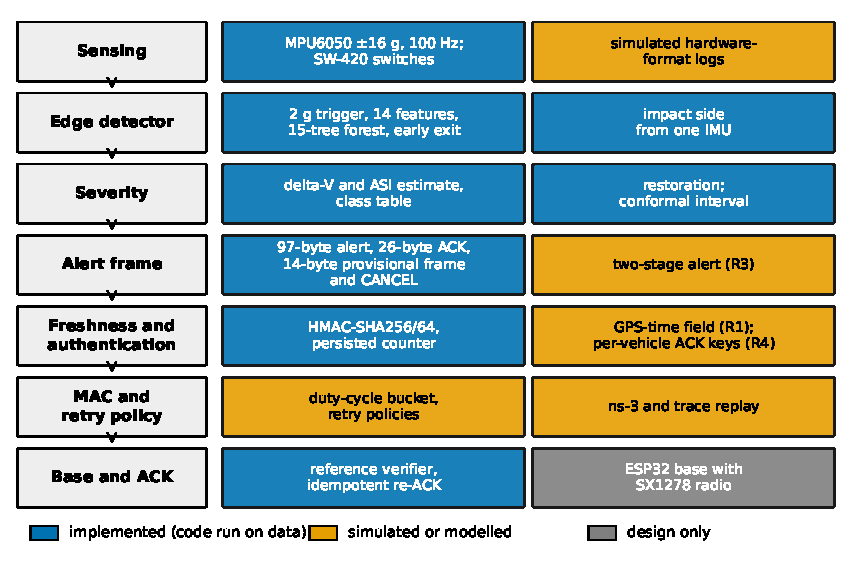
\includegraphics[width=\columnwidth]{figures/pp_arch.pdf}
\caption{Layered architecture with the status of each element (implemented, simulated or modelled, design only). Evidence labels of the results for each layer are given in the sections that follow.}\label{fig:arch}\end{figure}

\textbf{Constrained-node profile.} Every result is stated against one profile. \emph{Compute and memory:} an ESP32-class microcontroller with an SX1278 radio. The decision path (trigger, forest, framing, HMAC-SHA256, freshness, micro-confirm) was compiled for that target with the Espressif GCC toolchain: the forest is \RSixForestBytes{} bytes of constant data in flash, the HMAC code path is \RSixHmacCodeBytes{} bytes of code, and the stack of the micro-confirm check sums to \RSixStackChain{} bytes over its call chain (build artifacts, not board measurements; Section~\ref{sec:c8}). \emph{Link:} LoRa at 125 kHz with spreading factors 7 to 12, a 1\% duty limit (36 s of airtime per hour, enforced as an hourly allowance on one channel; no per-transmission off-time and no 433 MHz channel plan is modelled, Section~\ref{sec:c5}), 14 dBm transmit power with a 10 dB extra loss in the link budget. We read the 10 dB as path margin, not as transmit-side loss: a compliant dipole node radiates at most \RsevbPowerMaxDipole{} dBm (10 mW e.r.p.~\cite{gsr347}), so the stored link results assume up to \RsevbPowerExtraDb{} dB more margin than such a node has, about \RsevbPowerSfSteps{} spreading-factor steps, and are an optimistic bound on link margin. The protocol, security and duty-cycle results do not depend on transmit power, a 14-byte provisional frame, a 97-byte confirmed alert and a 26-byte acknowledgement. \emph{Energy:} datasheet currents only; no energy measurement. Hardware results are collected separately by the author and are not part of this paper.

\textbf{Data and splits.} The crash-test pulses of the National Highway Traffic Safety Administration (NHTSA) \cite{nhtsa} (\SevTests{} tests for the range study, \PoolN{} pooled records for the mode analysis) are split into development, validation and sealed folds. VZCrash \cite{vzcrash} is a naturalistic crash dataset (CC BY-NC 4.0, revision recorded in the supplement); it has no vehicle identifier, so its split is the one supplied and, for the audit, the de-duplicated split of Section~\ref{sec:c1}. The public LoRaWAN traces are the LoRaWAN at the Edge dataset (LoED) \cite{loed,loed_data20} and a LoRaWAN sniffer set \cite{sniffer} (both CC BY 4.0); the link is the device and the split is by device (hash of the device address), so no device is in both halves. A Brno urban measurement \cite{brno} is used descriptively. Gateway placement uses the Fatality Analysis Reporting System (FARS) crash files \cite{fars} and GeoNames \cite{geonames}. Every file was checked against the hash written in its preregistration (supplement, data sources). Thresholds were chosen on validation data only, and the test data were touched once per model.

\textbf{Preregistration, ledger and statistics.} \LedgerN{} hypotheses were preregistered in \LedgerVersions{} versions (V1 to V19, with addenda; H-R7-A3 of V18 is descriptive and has no verdict); \LedgerRun{} were run. Of these, \LedgerSupp{} are supported, \LedgerNot{} are not supported, \LedgerPartly{} are partly supported and \LedgerNotRun{} were not run (Table~\ref{tab:ledger}; the ledger with every row is in the supplement). The preregistrations are author-registered and time-stamped only by repository commits, not by an external registry. Each version has its own Holm family, so a $p$-value is adjusted only against the hypotheses of its own version and the families are never merged; \LedgerConfN{} hypotheses sit in a stated family, of which \LedgerConfSupp{} are supported (the rows that were not run enter with $p=1$, so this number exceeds the number run). A hypothesis is called supported only if its stated criterion holds and, in a family, the adjusted $p$ is below 0.05; a small $p$ with a missed effect size is not supported. Hypotheses added after results were seen (the repeated studies of V5, the Nessa-style baseline of V12 and the mirror-flip test L11 of V16) are marked and kept outside the confirmatory families or in a family of their own. Intervals are 95\% bootstrap intervals (resampling devices, events or runs, as stated), seed 42 and seeds 0 to 4 for repeated runs where they were run. A bootstrap $p$-value is (count + 1)/(resamples + 1) and has a floor. VZCrash has no vehicle identifier, so events from one vehicle may be dependent and the intervals are probably optimistic; the same test data were used in several versions, and no correction across versions was made. Each hypothesis has a data role: development (design choices, at most five logged iterations), held-out (scored once after a frozen, hashed configuration), sealed (a fold kept back until the freeze) or fresh (data that no earlier version used).
\begin{table}[t]\centering\caption{Hypothesis ledger by round (ANALYTICAL, counts of preregistered hypotheses; every row is in the supplement, with the Holm family of each version). Partly = some cells hold and others do not.}\label{tab:ledger}\footnotesize\setlength{\tabcolsep}{2pt}
\begin{tabular}{p{2.3cm}rrrrrr}\toprule
Round (versions) & Prereg. & Run & Supp. & Not supp. & Partly & Not run\\\midrule
Early studies (V1 to V5) & \LgAPre{} & \LgARun{} & \LgASupp{} & \LgANot{} & \LgAPartly{} & \LgANotRun{}\\
Release, redesign, paper (V7, V11 to V13) & \LgBPre{} & \LgBRun{} & \LgBSupp{} & \LgBNot{} & \LgBPartly{} & \LgBNotRun{}\\
Round 3 (V14) & \LgCPre{} & \LgCRun{} & \LgCSupp{} & \LgCNot{} & \LgCPartly{} & \LgCNotRun{}\\
Round 4 (V15) & \LgDPre{} & \LgDRun{} & \LgDSupp{} & \LgDNot{} & \LgDPartly{} & \LgDNotRun{}\\
Round 5 (V16) & \LgEPre{} & \LgERun{} & \LgESupp{} & \LgENot{} & \LgEPartly{} & \LgENotRun{}\\
Round 6 (V17) & \LgFPre{} & \LgFRun{} & \LgFSupp{} & \LgFNot{} & \LgFPartly{} & \LgFNotRun{}\\
Round 7 (V18) & \LgGPre{} & \LgGRun{} & \LgGSupp{} & \LgGNot{} & \LgGPartly{} & \LgGNotRun{}\\
Round 7b (V19) & \LgHPre{} & \LgHRun{} & \LgHSupp{} & \LgHNot{} & \LgHPartly{} & \LgHNotRun{}\\\midrule
All versions & \LedgerN{} & \LedgerRun{} & \LedgerSupp{} & \LedgerNot{} & \LedgerPartly{} & \LedgerNotRun{}\\
In a Holm family & \LedgerConfN{} & -- & \LedgerConfSupp{} & -- & -- & --\\\bottomrule\end{tabular}\end{table}

\textbf{Evidence labels.} MEASURED\_SOFTWARE: computed from a dataset. SIMULATED: produced by a simulation with stated assumptions. SIMULATED\_HW\_FORMAT: code run on simulated hardware-format logs. TRACE\_DRIVEN: measured link traces replayed in software. FORMAL: a proof or an exhaustive enumeration. ANALYTICAL: a formula. The assumptions of every simulation are listed in the supplement. No label claims a hardware measurement.

\textbf{Simulators and tools.} The custom simulator and ns-3 \cite{Riley2010_ns3} (version 3.48 with the lorawan module \cite{Magrin2017_ns3lora}, commit e45b4af) run the same alert scenarios. The module needed local changes: the receive-window delays are run-time variables, a sensitivity offset was added, and a null-pointer fault when the second receive window uses a frequency outside the known sub-bands was fixed. The patch is in the repository and the release archive lists it; \NsPatchRuns{} runs were repeated in the patched build and every output file was identical to the stored one. The ns-3 sensitivity tables were set to the custom simulator's values for the calibration; the calibration criterion was not met, so every cross-simulator statement is made under a calibration that did not reach its own target. Formal tools: Tamarin \cite{Meier2013_tamarin} \EnvTamarin{} with Maude \EnvMaude{} (symbolic Dolev-Yao model, node compromise by key reveal) and ProVerif \cite{Blanchet2016_proverif} \EnvProverif{}, run one lemma per process; a bounded model check of the retry and cancel protocol; and exhaustive enumeration of the frozen retry-policy code for $k=0$ to 6 consecutive losses (not timed automata and not the UPPAAL model checker). Software: Python \EnvPython{}, numpy \EnvNumpy{}, scipy \EnvScipy{}, scikit-learn \EnvSklearn{}; the pinned environment and the model files are in the repository.

\section{Results A: data and sensing}
\label{sec:resA}
\subsection{C1: benchmark audit}
\label{sec:c1}
VZCrash has \VzGroups{} groups of identical accelerometer arrays that cross the training, validation and test splits, holding \VzGroupEvents{} events (\VzCrashEvents{} crash events); \VzTestExact{} test events (\VzTestExactShare\%) have an identical array elsewhere. Of \VzNearScanned{} triggered test windows, \VzNearBoth{} (\VzNearShare\%) are identical to a training or validation window. A window duplicate is a triggered test window that is identical, sample for sample, to a training or validation window. Only test events were removed; the training and validation sets were not changed and the thresholds were chosen on the validation set as it is. The results are for this forest and not for the dataset authors' model. The forest's system recall falls from \VzRecSup{} on the supplied test events (\VzEvSup{}) to \VzRecNear{} on the de-duplicated events (\VzEvNear{}), and its recall at the 1\% false-alarm target falls from \VzROneSup{} to \VzROneNear{} (Fig.~\ref{fig:audit}, Table~\ref{tab:audit}). The audit is MEASURED\_SOFTWARE; the dataset authors acknowledged it by correspondence (the release and revision that credit it are to be cited by the author; supplement, data sources). The value \VzRecSup{} is the system recall (all crash events of the split) on the test split as supplied, at the validation threshold that maximises F1, with the duplicates in it; it is neither the recall of a naive window-level split nor a vehicle-grouped result. The unit of the split is the event, the release has no vehicle or trip identifier, and a vehicle-grouped split cannot be built. Removing exact copies alone leaves the recall at \VzRecExact{}; removing identical windows lowers it to \VzRecNear{}; this fall is consistent with leakage but also with removing easy events, because the test population changes. A naive random re-split of the training and validation events, made without the test set and illustrative only, gives \VzRecNaive{}, close to the supplied value; it is a different population and not a test of leakage. The audit is a reusable procedure (exact array hashing; window-identity matching with a correlation above 0.999 and a maximum difference below 0.01 g; the 2 g trigger and the 16 g clip rules); the supplement gives the procedure and the code. The wider concern is stated in Section~\ref{sec:related}: no duplicates were found in UCI HAR (\RFiveHar{} test windows) or SisFall, so the finding is specific to VZCrash.
\begin{figure}[t]\centering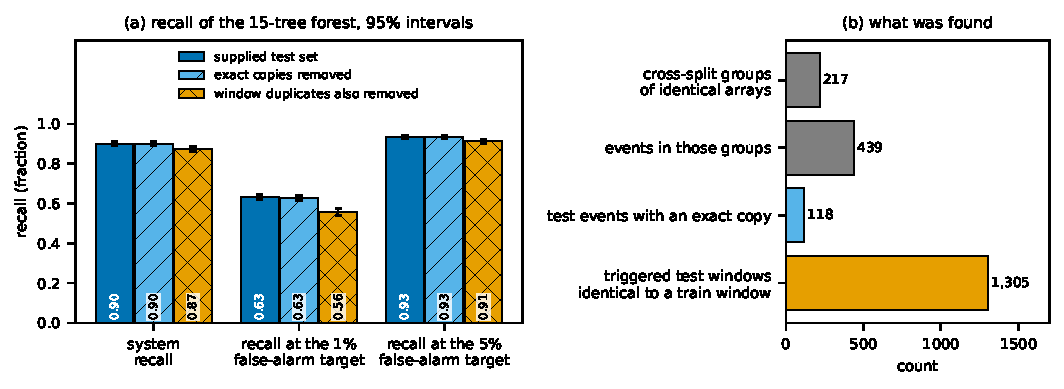
\includegraphics[width=\columnwidth]{figures/vf_audit.pdf}
\caption{C1: (a) recall of the 15-tree forest on the supplied VZCrash test set, without exact copies and without window duplicates; (b) counts found by the audit (MEASURED\_SOFTWARE).}\label{fig:audit}\end{figure}
\begin{table}[t]\centering\caption{C1: effect of removing duplicates from the VZCrash test set (MEASURED\_SOFTWARE). The last row is a naive random re-split of the training and validation events, not the test set (descriptive).}\label{tab:audit}\small\setlength{\tabcolsep}{3pt}
\begin{tabular}{p{3.0cm}rrr}\toprule
Test set & Events & System recall & Recall, 1\% target\\\midrule
Supplied & \VzEvSup{} & \VzRecSup{} & \VzROneSup{}\\
Exact copies removed & \VzEvExact{} & \VzRecExact{} & \VzROneExact{}\\
Duplicates removed & \VzEvNear{} & \VzRecNear{} & \VzROneNear{}\\
Random re-split (illustrative) & \VzNaiveN{} & \VzRecNaive{} & \VzROneNaive{}\\\bottomrule\end{tabular}\end{table}

\subsection{C2: sensing requirement}
For each of \SevTests{} NHTSA tests, the delta-V of a modelled sensor chain (range, rate, clipping) was compared with the reference delta-V. At $\pm$16 g and 100 Hz, \DvSixteen\% of tests are within $\pm$10\%; at $\pm$32 g, \DvThirtyTwoA\% (100 Hz) and \DvThirtyTwoB\% (200 Hz); at $\pm$64 g, \DvSixtyFourA\% and \DvSixtyFourB\%; \DvSettingsMeet{} of \DvSettingsAll{} range and rate settings reach 80\%. By crash mode, the smallest range that meets the 0.80 rule is $\pm$\ModeFrontReal{} g for frontal-barrier tests (\ModeFrontN{} records) and $\pm$\ModePoleReal{} g for pole tests (\ModePoleN{} records); no configuration meets the rule for side (\ModeSideN{} records) or other tests (\ModeOtherN{} records) (Table~\ref{tab:modes}, Fig.~\ref{fig:heat}). The pulses are channels at crash-test sensor locations, not a node mounting, and records from one test are not independent, so the intervals are optimistic.
\begin{figure*}[t]\centering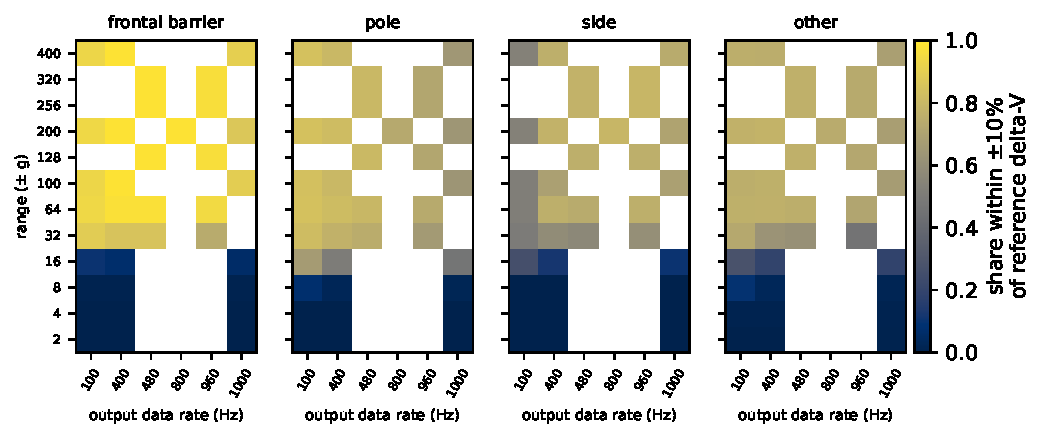
\includegraphics[width=\textwidth]{figures/pp_heat.pdf}
\caption{C2: share of tests with delta-V within $\pm$10\% of the reference, by crash mode, accelerometer range and output data rate (best of eight parts per cell; blank = no part offers that setting). MEASURED\_SOFTWARE on the pooled records.}\label{fig:heat}\end{figure*}

\emph{Stress-test check, refitted.} A synthetic stress test asks whether pulses from a generator give the same smallest range as the real records. The original check fitted its generator to all \PoolN{} records, so it was in-sample. It was refitted on the development fold only (\RefitNFit{} records) and gated against the held-out records (\RefitNGate{}). The modes that passed the gate are \RefitPassed{} (the other mode passed the gate, but no configuration meets the rule for the real records, so there is no range to compare). For frontal-barrier pulses the synthetic range is $\pm$\RefitFrontSyn{} g, equal to the real one (step difference \RefitFrontStep{}); the verdict is \RefitVerdict{} (Holm-adjusted $p=$ \RefitHolm{}), the same as the original verdict (\OrigVerdict{}). The largest held-out Kolmogorov-Smirnov statistic for frontal barrier is \RefitKsFront{} against the gate of 0.20, so the pass is narrow. The pole mode failed the gate and is not tested; its synthetic range is exploratory. The label is SIMULATED.
\begin{table}[t]\centering\caption{C2: smallest range meeting the 0.80 rule, real and refitted synthetic (100 Hz; SIMULATED for the synthetic column).}\label{tab:modes}\small
\begin{tabular}{lrrl}\toprule
Mode & Records & Real & Refit synthetic\\\midrule
Frontal barrier & \ModeFrontN{} & $\pm$\ModeFrontReal{} g & $\pm$\RefitFrontSyn{} g (passed gate)\\
Pole & \ModePoleN{} & $\pm$\ModePoleReal{} g & $\pm$\RefitPoleSyn{} g (failed gate)\\
Side & \ModeSideN{} & none & --\\
Other & \ModeOtherN{} & none & not compared\\\bottomrule\end{tabular}\end{table}

\emph{Restoration at $\pm$16 g.} A pulse-fit restoration reduces the median delta-V error at $\pm$16 g to \RestMedRest\% from \RestMedPlain\% (plain) and \RestMedSpl\% (spline), but the 90th-percentile error is \RestPNinetyRest\% against \RestPNinetyPlain\% (plain) and \RestPNinetySpl\% (spline), so it is worse in the tail. At $\pm$32 g the gain over plain is \RestThirtyTwoGain{} points with an interval upper end of \RestThirtyTwoUpper{}, and against spline the interval (from \RestThirtyTwoSplLo{} to \RestThirtyTwoSplHi{}) includes zero; at $\pm$64 g the difference is \RestSixtyFourDiff{} and includes zero. Restoration is a limited fix at $\pm$16 g, not a method claim; spline is the baseline (figure in the supplement).

\section{Results B: detection}
\label{sec:resB}
\emph{C3: compact detector.} A sweep of \PfourConfigs{} forest configurations picked, on validation data, a forest with 16-bit thresholds that has a flash estimate of \PfourFlash{} bytes against \PfourRefFlash{} bytes for the reference (\PfourRatio\% of it). Validation average precision is \PfourValAp{} against \PfourRefValAp{}; on the de-duplicated test events the loss is \PfourApLoss{}. Recall at the 1\% target is \PfourRecOne{} against \PfourRefRecOne{} (Fig.~\ref{fig:p4a}). The flash figure is ANALYTICAL (node count times bytes per node); no microcontroller build was measured. The only comparison is between the reference forest and its own compact variant; no simple baseline (a peak threshold, logistic regression, boosting or a small network) was run for this comparison, and VZCrash has few crash events, so the intervals matter.
\begin{figure}[t]\centering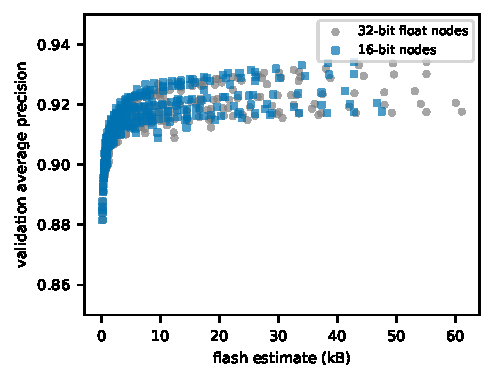
\includegraphics[width=0.85\columnwidth]{figures/pp_p4a.pdf}
\caption{C3: flash estimate against validation average precision for \PfourConfigs{} forest configurations (MEASURED\_SOFTWARE; flash ANALYTICAL).}\label{fig:p4a}\end{figure}

\emph{Other detector results.} Trigger-aware training and selection did not raise system recall at a fixed false-alarm rate beyond the interval (baseline recall at the 1\% target \TrigBaseRecall{}); this is a negative result. At a crash prevalence of one in five thousand, the positive predictive value is \PrevOne\% at the 1\% target and \PrevFive\% at the 5\% target (ANALYTICAL): the detector alone would send mostly false alarms, which is why a confirmation stage and the retraction of provisional alarms matter. The early-exit rule decides about \EarlyTimeOne{} s earlier than the full window at the 1\% target (timing is the window length, SIMULATED); its recall gain over a single full-length forest, averaged over five seeds, is \EarlyGainOne{} at the 1\% target and \EarlyGainFive{} at 5\%, and the gain is not an early-exit effect.

\section{Results C: protocol, alert and deployment}
\label{sec:resC}
\subsection{C4: authenticated alert protocol}
\label{sec:c4}
\textbf{Tamarin.} Figure~\ref{fig:proto} lists the lemmas. In the shared-key design (M0) one node key is shared by the cell and the acknowledgement names only the alert field; Tamarin finds that a node holding the key can forge an acknowledgement that makes another vehicle stop its retries. With a key derived per vehicle and an acknowledgement bound to the vehicle and the alert field (M1), alert authenticity, acknowledgement authenticity and the absence of cross-vehicle suppression are proved. In the freshness model (an alert is accepted in its own or the next epoch, once, per vehicle and field) the window, at-most-once and no-double-acceptance-after-a-car-reboot properties are proved. A replay after a base reboot is possible by design, because the seen-set is lost; Tamarin finds the trace. The lemma that alert identifiers are not reused after a car reboot was tried in three formulations and was not decided within the limits. The label is FORMAL: a symbolic model with perfect cryptography, not the implementation. The proofs cover the protocol at the level of the stated message structure. The abstractions that separate the models from the byte layout (a vehicle as one name, the freshness identifier as one value, a window of two epochs where the simulations use \ROneWindow{} s, an unbounded seen-set, perfect cryptography, letters for type fields, and the lookup of a micro frame by vehicle and provisional tag) are listed in one table of \FrameAbstractRows{} rows in the supplement; no formal model covers the freshness field of the 14-byte provisional frame or the 16-bit short node identifier.
\begin{figure*}[t]\centering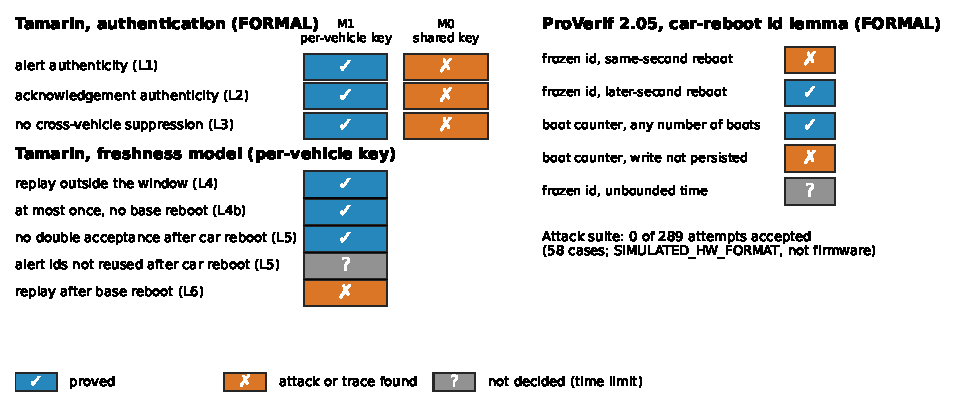
\includegraphics[width=\textwidth]{figures/vf_proto.pdf}
\caption{C4: formal results (FORMAL). M1 = per-vehicle key, M0 = shared cell key. The attack suite is SIMULATED\_HW\_FORMAT and does not test firmware. Reruns with times and memory are in the supplement.}\label{fig:proto}\end{figure*}

\textbf{Second prover and the boot counter.} ProVerif finds an attack on the frozen design when a car reboots inside the global positioning system (GPS) second of an earlier alert: the sequence counter restarts and two different alerts carry the same identifier. It proves, in the symbolic model, for any number of boots and without a timing assumption, that identifiers are not reused when the car keeps a boot counter in non-volatile memory and adds it to the identifier; a control whose write does not persist fails. The frozen design is therefore safe only if a reboot takes at least one second, and only in a bounded model (the unbounded ordered-time formulation did not terminate in either prover). We adopt the boot counter as the recommended design. It costs one non-volatile write per boot, which is the write that the boot-epoch freshness design already counts, so the saving of about \ROneRatio{} times in flash writes at 100 alerts and 12 boots per car and year, against persisting the counter of every alert in the car and the base, remains (ANALYTICAL). The alert frame has room for the counter; the 14-byte provisional frame would grow to 15 bytes, and the airtime does not change (\FlashAirSeven{} ms at SF7 and \FlashAirNine{} ms at SF9 for 13 to 15 bytes). The proofs use an unbounded boot counter; the 8-bit truncation of the counter in the 15-byte frame (it wraps after 256 boots between two heard frames) is outside the proof. The supplement gives the byte layout of every frame, with the freshness field (GPS seconds and a sequence in the second) and the boot counter (four bytes in the alert, its low byte in the 15-byte provisional frame); the layout is a design proposal, checked by tests against the encoders where an encoder exists, and no firmware implements it.

\textbf{Bounded model, timing and attacks.} A bounded model of the protocol (send, retry, signed acknowledgement, cancel, two-stage provisional frame, counter and replay window, re-acknowledgement, reboots and an attacker; \BmcStates{} reachable states at depth \BmcDepth{}, \BmcProps{} properties) shows that a retry and a replay look the same to the base: a strict verifier that rejects every repeated counter leaves a car whose acknowledgement was lost retrying without receiving one, and acknowledging a remembered repeat again without processing it again removes the conflict. It also gives a counterexample to the property that a delivered cancel is never lost by reordering, which remembering a cancel for a counter not yet seen removes (ANALYTICAL: a model, not the implementation). Exhaustive enumeration of the frozen retry-policy code for $k=0$ to 6 consecutive losses (\TimedRuns{} duty-cycle runs) shows that the worst-case delivery time of the adaptive table is not longer than that of quick retries for every $k$, with no breach of the hourly allowance; after six lost uplinks the table delivers within the 10 s deadline in \TimedDOneSix{} s and quick retries do not (FORMAL, single link). In the bounded model, one forged event-level acknowledgement from a holder of the shared key stops a fraction \RFourShared{} of the vehicles; with per-vehicle keys one compromised node stops only itself (\RFourPer{} for three vehicles), at one key derivation per new vehicle identifier and no extra bytes. The repository's attack suite of \SuiteTotal{} cases and the simulated scenarios behave as designed: \SuiteAccepted{} of \SuiteAttempts{} attack attempts were accepted (the suite and the code are the author's own and the firmware was not tested, so this is a regression check and not evidence of resistance). A GPS-time freshness field with a \ROneWindow{} s window accepts at least \ROneAvail\% of valid alerts after a car reboot in simulation, but the replay bound inside the window needed a ring larger than the alerts per window (replay rate \ROneRate{} at the held-out burst with \ROneRing{} entries), which missed its bound. For an 8-byte tag, $2^{\ForgeOne}$ forgery attempts give a success probability of $10^{-6}$ and the expected number of attempts is $2^{\ForgeExp}$ (ANALYTICAL).

\textbf{Quarantine and flood containment (R6-3b, FORMAL, bounded).} A rule that counts frames per claimed vehicle identifier before the tag is checked lets an attacker without any key move a victim into quarantine: a bounded exhaustive exploration in Python (three claimed identifiers, six one-minute slots, up to four attacker frames per slot, the counters of the round-5 flood model) reaches quarantine of the victim with \RSixQuarFrames{} frames in one slot. The base code checks the tag before anything else and has no quarantine counter, so this is an attack on a rule as modelled and not on the implementation. The design fix is two counters: frames that fail the tag may only raise a per-cell rate limit and never quarantine a vehicle, and per-vehicle quarantine applies only to authenticated misbehaviour, counted after verification. With the counter after verification no frame of a key-less attacker reaches the victim's counters; this holds by construction of the rule, and the exploration confirms it for the bound. The result is for the modelled mechanism and bound only; the symbolic provers were not used for this part.

\textbf{Duty-budget exhaustion and the reserved budget (rounds 7 and 7b).} An attacker that suppresses the acknowledgements makes the node spend airtime on retries. This attack class is known: energy-depletion and denial-of-service attacks on LoRaWAN, including attacks on confirmed transmission that rely on the duty-cycle limit \cite{R7Mikhaylov2019,R7Nafees2020,R7EdaLora2026,R7MacDos2023}, are prior work, and we do not claim the attack. Nodes without keys cannot use up the base's downlink duty budget with confirmed frames, as in that attack class: in the reference base a frame whose tag fails gets no acknowledgement and is rejected before any state changes (cell-level rate limiting is the design for such frames), whereas a keyless replay of a captured valid frame is re-acknowledged each time and can consume the base's downlink budget unless two limits are on, the re-acknowledgement interval and the downlink budget. We state them as deployment requirement R-REACK, with the values of the replay-flood study: no re-acknowledgement of the same event sooner than the shortest legitimate retry spacing (\RsevdIntervalSeven{} s at SF7, \RsevdIntervalEight{} s at SF8, \RsevdIntervalNine{} s at SF9), and a downlink token bucket that refills at the \RsevdDutyPct\% duty cycle with a capacity of \RsevdCapacity{} s (it started at \RsevdInitial{} s in the study). With the limits off, \RsevdRate{} replays a second for \RsevdDuration{} s of one valid alert at SF7 drew \RsevdOffReacks{} re-acknowledgements and \RsevdOffAirtime{} s of airtime, the budget ran out and a genuine alert at 100 s was accepted but not acknowledged; with them on, \RsevdOnReacks{} and \RsevdOnAirtime{} s, and the genuine alert was acknowledged. The limits stop the starvation but not the waste (the replays still spent \RsevdOnShare\% of the starting budget; a stricter limit was not evaluated). The reference verifier has both limits off by default; a new reference configuration turns them on without touching any frozen file. The ns-3 gateway model does not check tags and has no such limit. What this paper adds is the defence for a two-stage alert, a bounded model check with a control, and preregistered results under India's rules (the 10\% duty cycle is the main deployment regime; the 1\% allowance is the stricter case). The shipped policy caps the flash at four tries and the confirm at four, so one fully suppressed event costs the node \RsevNodeAirSfSeven{} s at SF7 and \RsevNodeAirSfNine{} s at SF9, while the attacker, who only has to jam each 26-byte acknowledgement, spends at most \RsevAttackRatioSfSeven{} of that airtime (ANALYTICAL). Spending a trailing-hour allowance of 1\% takes \RsevNstarOneSfSeven{} such events in one hour at SF7 (one every \RsevGapSfSeven{} s) and \RsevNstarOneSfNine{} at SF9 (\RsevNstarTenSfSeven{} and \RsevNstarTenSfNine{} at 10\%). We did not measure how often a detector produces such a rate, so this is a regime and not a measured attack. Under a per-transmission off-time of 10\% the effect is immediate: the flash retries lock the sub-band and the confirm starts \RsevTtenOldDelaySfSeven{} s late at SF7 and \RsevTtenOldDelaySfNine{} s late at SF9. The reserved policy keeps an airtime reserve, lets only the confirm, micro-confirm and cancel frames spend it, withdraws flash tries when the follow-up is due, and under an off-time admits a flash try only if its off-time ends before the follow-up is due. \emph{Registration V18 (k = 1).} The reserve for one event (four confirm copies and one micro-confirm) was preregistered with a 99\% target. In the simulation at the load that exhausts the shipped policy at 1\%, it keeps the follow-up on time in \RsevAoneRateOneResSfSeven\%, \RsevAoneRateOneResSfEight\% and \RsevAoneRateOneResSfNine\% of the runs at SF7, SF8 and SF9 (the shipped policy: \RsevAoneRateOneOldSfSeven\%, \RsevAoneRateOneOldSfEight\% and \RsevAoneRateOneOldSfNine\%), so hypothesis H-R7-A1 is not supported; it holds in every run at 10\% and under the off-time. Earlier follow-ups spend the reserve. \emph{Registration V19 (k = 4).} After that run, a post-run sweep showed that a reserve for four events reaches 100\%. Because this size was chosen from the round-7 data, we preregistered it (V19) and tested it on fresh seeds, with the thresholds of V18 unchanged; this is a confirmation and not a blind test. H-R7b-1 is supported: the follow-up is on time in at least \RsevbWorstLower\% of runs (lower 95\% limit) in all \RsevbCellsFeasible{} cells (SF7 to SF9; the 1\% and 10\% allowances and the 10\% off-time; p = \RsevbPOne{}), and at the 1\% allowance the reserve for one, two, three and four events gives \RsevbOneRateSfSeven, \RsevbTwoRateSfSeven, \RsevbThreeRateSfSeven and \RsevbFourRateSfSeven\% at SF7 (descriptive). The reserve for four events takes \RsevReserveFourShareSfSeven\% of the 1\% allowance at SF7 and \RsevReserveFourShareSfNine\% at SF9. H-R7b-2 is not supported: without an attack, delivery on the measured traces falls by \RsevbBenignHTenDelta{} percentage points in the high-loss group under the 10\% off-time (\RsevbBenignFailCells{} of \RsevbBenignCells{} cells, both schemes), against a bound of 1, because the time reserve admits \RsevTtenFlashTriesSfSeven{} flash tries instead of four; under the hourly allowance the fall is \RsevbBenignHHourDelta{} points, and the median time to an alert stays within the 10\% bound in every cell. The fall does not change with the size of the reserve (descriptive curve for one to four events), because the replay runs each event with a fresh duty state; a cost that grows with the reserve under sustained load was not run. \emph{Bounded model check.} An enumeration with up to five earlier events (FORMAL, bounded; the abstraction has a window of 70 steps and three allowances) finds no violation of the reserve rule and no late follow-up while the reserve is intact for the reserves of one and four events, and \RsevbFormOldCond{} late runs for the shipped policy; the guarantee is conditional on the reserve being intact: the reserve for one event fails with \RsevbFormMOneFirst{} earlier events, and the reserve for four events with \RsevbFormMFourFirst{}. The control that V19 registered (the one-event reserve fails with at most three earlier events) was not met as worded: in this window the one-event reserve fails from \RsevbFormMOneFirst{} earlier events, so the control separates the two reserves only at the bound of four; the registered expectation for the four-event reserve (failure from four) was also off by one (supplement, deviations table). An earlier enumeration with a window of 30 steps and at most two earlier events (the bounds of the V18 run, after an attempt with a window of 10 steps that was too short to show a limit) found the one-event reserve failing with \RsevFormMinEarlier{} earlier events. The models are abstractions of the queue, not of the radio.

\textbf{Unlinkable pseudonymous ids (round 7).} In the layout the vehicle id, the boot counter and the alert counter are in clear, so an observer can link all alerts of a vehicle. The design replaces the id by a pseudonym, the leading $L$ bytes of HMAC-SHA256 under the per-vehicle key of a label, the boot counter and the alert counter (the sequential scheme of \cite{R7Pelissier2024} with a keyed function), removes boot and counter from the clear (the base recovers them from the window entry that matches), encrypts the position and payload, and lets the tag cover boot and counter as unsent associated data. The base keeps a window of the next 16 pseudonyms per vehicle, finds the vehicle through a hash index, and applies the boot-counter rule, the seen-set and the per-vehicle quarantine to the resolved id; a frame that does not resolve or fails the tag triggers only cell-level rate limiting. In ProVerif the diff-equivalence holds for two alerts and for an unbounded number of alerts: a network attacker that listens, replays and injects cannot tell two alerts of one vehicle from two alerts of two vehicles. The fixed-id design fails with a trace, and so does a variant that sends the boot counter in clear (FORMAL; H-R7-B3 supported). The earlier lemmas hold with the pseudonym: authenticity, unique ids with the boot counter, micro-confirm binding with the index and no framing by the quarantine counter in ProVerif, and the freshness, anti-replay and reboot lemmas in Tamarin (each run at most \RsevTamExecS{} s). For the quarantine, ProVerif proves the non-injective no-framing form and reports the injective form false with a trace of two base threads that both read the seen-set before either inserts; a Tamarin model in which the seen-set check and insert are one step verifies both forms, and the controls without a seen-set and with a strike before the tag check fail as expected. So the quarantine rule keeps its no-framing property with pseudonyms if the base applies the seen-set atomically, and not otherwise (a separate small model; the window advance and reboots are not in it). The reference base code in the repository is a sequential, single-threaded loop with no lock or thread anywhere (a scan of \RsevcAtomicFiles{} source files finds no concurrency primitive), so the check and the insert are atomic there only by construction, and nothing enforces it; there is no base server. We therefore state it as a design requirement for any base: resolution, tag check, seen-set check and insert, and the strike are one critical section per resolved vehicle (one frame loop fed by all gateways, or a per-vehicle lock), and the quarantine lemma holds only with it. Resolving a frame takes at most \RsevBoneWorstUs{} microseconds in Python and \RsevBoneCUs{} in C for 1,000 vehicles and a window of 16 (MEASURED\_SOFTWARE; H-R7-B1 supported); the frame that follows a reboot costs \RsevBoneResyncMs{} ms (a linear scan; a table of the pseudonyms of the next three boot values for every vehicle would turn it into a lookup: \RsevbRebootEntries{} entries and about \RsevbRebootBytes{} bytes for 1,000 vehicles, rebuilt for one vehicle after each match; a design note, ANALYTICAL, not implemented). The pseudonym equals an entry of another vehicle's window with probability \RsevBtwoLTwo{} per frame at the 2 bytes of the flash and \RsevBtwoLFour{} at the 4 bytes of the alert, above the bound of $10^{-6}$ (H-R7-B2 is not supported; \RsevBtwoLMeet{} bytes would meet it). The tag decides a collision, so it costs one extra tag check and not a wrong attribution; at 5 bytes the probability is \RsevbCollFive{} per frame, below the bound, and the extra byte adds \RsevbExtraByteAckSeven{} ms to the acknowledgement at SF7 and \RsevbExtraByteAckNine{} ms at SF9 (none to the 97-byte alert at SF7 to SF9; ANALYTICAL; the verdict of H-R7-B2 is unchanged); without the counter in the tag, two entries of one vehicle with equal pseudonyms desynchronised the window in our C test, which is why the tag covers it. Unlinkable ids do not hide position, timing or the radio fingerprint, and an attacker that holds a vehicle key is outside the model; responders get the position from the base, not from the air. Frame sizes do not change; a 16-byte authentication tag on the alert would add \RsevAeadExtraSfSeven{} ms at SF7 and \RsevAeadExtraSfNine{} ms at SF9. The routine takes \RsevFpText{} bytes of code on the ESP32 target (compile only) and \RsevFpStack{} bytes of stack on its deepest call path. Against \cite{R7Pelissier2024}, which argues unlinkability informally for a passive observer, this adds a formal model with an active attacker and the checks together with replay protection and quarantine.

\subsection{C5: two-stage alert}
\label{sec:c5}
\textbf{Design.} At the early-exit decision the node sends a 14-byte provisional frame, which carries ``crash detected, severity pending'' and no severity class. At the full-window decision it sends the full alert, or an authenticated cancel (three transmissions) if the full window does not alarm. The reason for the missing class is that a severity class taken from a window truncated at 50 ms agrees with the full-window class for only \TThreeNhtsaFifty\% of the \TThreeNhtsaN{} frontal NHTSA pulses (\TThreeNhtsaHundred\% at 100 ms and \TThreeNhtsaTwo\% at 200 ms).

\textbf{Detection side (MEASURED\_SOFTWARE).} On the de-duplicated VZCrash test events the provisional decision comes a median of \TThreeEarlier{} ms before the full window; \TThreeRetract\% of provisional alarms are withdrawn at the 1\% target (95\% upper limit \TThreeRetractHi\%) and \TThreeFiveRetract\% at the 5\% target. The VZCrash class agreement (\TThreeVzClass\% over \TThreeVzN{} events) carries no information because almost all of those events are in the lowest class.

\textbf{Link side.} Table~\ref{tab:r3} gives the three clauses in three link models: the custom simulator (SF7), measured traces (SF7 timing) and ns-3 (SF7 and SF9, both sensitivity settings, extra loss of 0 to 0.6, \NsRuns{} runs). The provisional alert arrives \RThreeEarly{} s earlier in the custom simulator, \TOneEarlier{} s on traces and \NsEarlySfSeven{} s (SF7) and \NsEarlySfNine{} s (SF9) in ns-3. Delivery is not worse than single-stage by more than two points anywhere. The extra airtime is \RThreeAir\% in the custom simulator, \NsAirLoSfSeven{} to \NsAirHiSfSeven\% at SF7 in ns-3 and \NsAirHiSfNine\% at SF9, so the 40\% bound holds at SF7 and fails at SF9 (the bound is a design budget fixed in the preregistration, not a regulatory value). The extra airtime includes the three cancel transmissions and the retries of the provisional frame, so it is larger than the share of one frame: the provisional frame alone costs about \FlashShareSeven\% of the alert's airtime at SF7 and about \FlashShareNine\% at SF9. The ns-3 verdict is \NsVerdict{} (\NsSupported{} of 8 tests supported), and the SF9 airtime result is reported with it. The earlier-arrival figure is set by the window length and the early-exit time, so it is the same in all three link models: it is a design property and not a link finding. The retraction share is a detector property and is repeated in every column. The airtime figures are per triggered test event at the prevalence of the test set and exclude the load of false alarms in deployment (at a crash prevalence of one in five thousand almost every provisional frame would be a false alarm; Section~\ref{sec:resB}); the earlier-arrival figures are differences in arrival time, and the detector-side median above is a difference in decision time, so they differ. A bench run of this alert is the main item that only hardware can settle.

\textbf{Duty model and lockout.} Every simulation and replay here enforces an hourly allowance of airtime; none enforces a per-transmission off-time, and in ns-3 the module's sub-band duty is set to 1. In a region that enforces an off-time on one sub-band shared by all frames, a flash of airtime $A_f$ that starts at $s_f$ blocks the next frame until $s_f + A_f/d$, with $d$ the duty fraction. The confirm, due at $T_F=$ \DutyDue{} s, is then delayed by $(s_f + A_f/d - T_F)^+$, and it is not later than in the single-stage alert if and only if $A_f \le d\,(T_F - s_f)$ (ANALYTICAL; a condition from the stock ns-3 off-time formula, derived in the supplement). At 1\% the largest admissible flash airtime is \DutyCritMs{} ms, less than the airtime of any frame of 7 bytes or more, so the flash would delay the confirm at every spreading factor (the 14-byte flash blocks the sub-band for \DutyLockSeven{} s at SF7 and \DutyLockNine{} s at SF9); at 10\% the condition holds up to SF\DutyMaxSfTen{}. Because the module's sub-band duty is 1, \DutyStoredShare\% of the stored two-stage events at SF7 sent the confirm inside that interval, so the stored delivery and airtime results do not transfer to such a region. The Indian rules for 433.05 to 434.79 MHz allow 10 mW e.r.p. at a duty cycle of at most 10\% with no bandwidth limit, which covers LoRa at 125 kHz; they define the duty cycle over an observation interval that they do not state and give no channel plan~\cite{gsr347}. The evaluation used a 1\% hourly allowance, stricter than the 10\%. Under a per-transmission reading of the 10\% the condition holds up to SF\IndiaMaxSf{}, so the two-stage alert stays feasible in India under either reading (the load gate below still limits it to SF7); under a strict 1\% per transmission, as in some other regions, no frame fits and the stored two-stage results do not transfer. A confirm sent on a second channel would not be delayed. The simulations use 14 dBm with a 10 dB extra loss. We take the conservative reading, that the 10 dB is path margin: a dipole node then has to transmit at most \RsevbPowerMaxDipole{} dBm, which removes up to \RsevbPowerExtraDb{} dB of margin (about \RsevbPowerSfSteps{} spreading-factor steps at the simulators' sensitivity step; ANALYTICAL, no simulation was rerun at the lower power). The link results are therefore an optimistic bound on margin; the protocol, security and duty-cycle results do not use transmit power.

\textbf{Retry queue.} In the evaluated policies (r3t, r6m and the trace replays) the node keeps one FIFO queue per event: the provisional frame is retried until it is acknowledged or four tries are used, and only then is the confirm or the cancel sent; the confirm does not replace the flash, and a cancel is sent whether or not the flash was delivered. Preemption (withdrawing the remaining flash tries when the full decision is ready) is a design recommendation. It saves no airtime at SF7 to SF9, because all four tries end before the confirm is due (the last at \PreemptEndNine{} s at SF9), and \PreemptSaveTen{} s per event with an unacknowledged flash at SF10 (ANALYTICAL). An exhaustive enumeration of \PreemptCases{} cases (FORMAL, bounded, untimed) shows that preemption adds no end state, and that the base keeps the provisional state with no further frame only if every frame of the final stage is lost, with or without preemption; a base-side timeout would remove that state and is not in the code.
\textbf{Reserve and gating rule (round 7).} The queue above is the shipped policy. With the reserved-budget policy of Section~\ref{sec:c4} the flash is a low-priority frame: under the hourly allowance it is sent only while the reserve stays intact, and under a per-transmission off-time only while its off-time ends before the confirm is due, so the lockout of the previous paragraph cannot delay the confirm. The link-aware gating rule re-derived with the reserve keeps both gates: the load gate does not depend on the reserve, and the lockout gate is enforced by the node for each event (descriptive, H-R7-A3). The spreading factor at which the two-stage alert is enabled stays SF7. Under the off-time the reserve admits \RsevTtenFlashTriesSfSeven{}, \RsevTtenFlashTriesSfEight{} and \RsevTtenFlashTriesSfNine{} flash tries at SF7, SF8 and SF9 and none from SF10.

\begin{figure}[t]\centering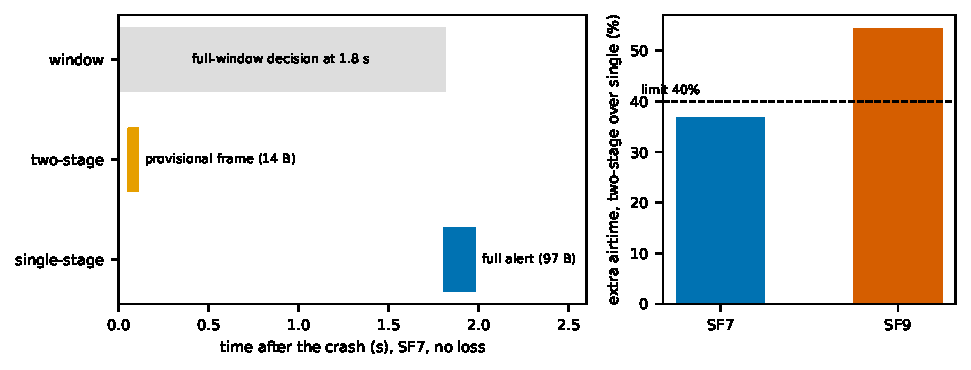
\includegraphics[width=\columnwidth]{figures/pp_r3.pdf}
\caption{C5: timeline of the single-stage and two-stage alerts at SF7 without loss (left; SIMULATED) and extra airtime of the two-stage alert in ns-3 (right; SIMULATED, largest over four loss levels and two settings).}\label{fig:r3}\end{figure}
\begin{table}[t]\centering\caption{C5: the three clauses of the two-stage alert in three link models.}\label{tab:r3}\small
\begin{tabular}{p{2.4cm}p{1.2cm}p{1.2cm}p{1.1cm}p{1.1cm}}\toprule
Clause & Custom (SF7) & Traces (SF7) & ns-3 SF7 & ns-3 SF9\\\midrule
(a) earlier by, s & \RThreeEarly{} & \TOneEarlier{} & \NsEarlySfSeven{} & \NsEarlySfNine{}\\
(b) retracted, \% & \RThreeRetract{} & \TThreeRetract{} & \RThreeRetract{} & \RThreeRetract{}\\
(c) extra airtime, \% & \RThreeAirMax{} & \TOneAirL{} to \TOneAirH{} & \NsAirHiSfSeven{} & \NsAirHiSfNine{}\\
(c) smallest delivery difference & \RThreeDelMin{} & \TOneDelH{} (group H) & \NsDelMinSfSeven{} & \NsDelMinSfNine{}\\
Verdict & supported & supported & holds & clause (c) fails\\\bottomrule\end{tabular}\end{table}

\subsection{C6: evaluation of retry policies}
\label{sec:c6}
\textbf{Custom simulator against ns-3.} A loss-adaptive retry table (D1) was designed from a diagnosis of the severity table's failure and tested once on \CellsN{} held-out cells of the custom simulator and then run on the same cells in ns-3. In the custom simulator it delivers \XCustomDOneGain{} more critical alerts within 10 s than the severity table at loss of 40\% or more; in ns-3 the same code delivers \XNsDOneGain{} more. The simulators disagree on whether D1 is never worse than the severity table by more than one point (smallest cell \XCustomMinCell{} against \XNsMinCell{}, with \XNsCellsFail{} of \CellsN{} ns-3 cells below it), so the verdict is simulator-dependent. In ns-3, quick retries deliver \XNsQuick{} against \XNsDOne{} for D1, while in the custom simulator they deliver \XCustomQuick{} against \XCustomDOne{}. The calibration did not reach its criterion, so the verdict is stated as dependent on the simulator and not as a finding about the radio.

\textbf{Measured traces.} The same policies were replayed, as single-link reductions without a crowd, on measured loss sequences from LoED. The held-out half has \TOneN{} devices (\TOneNL{} with loss under 10\%, \TOneNM{} between 10\% and 40\%, \TOneNH{} with 40\% or more, \TOneShareH\% of the devices). On links with loss of 40\% or more, delivery within 10 s is \TOneDelDOne\% for D1, \TOneDelQuick\% for quick retries, \TOneDelPOne\% for the severity table, \TOneDelKhan\% for the LoRaWAN-style rule and \TOneDelNessa\% for the Nessa-style rule (Fig.~\ref{fig:sim}); the best baseline minus D1 is \TOneDiffL{}, \TOneDiffM{} and \TOneDiffH{} in the three groups. A control that retries at once, with no hold and no spacing, delivers \TOneDelZ\% on those links, more than D1. The control respects the same 10 s deadline (\ZLate{} late deliveries) and its airtime is within the limit: one alert can use at most \ZMaxAir{} s, \ZMaxShareOne\% of the hourly allowance of the 1\% limit. The finding is limited to these single-link replays, which carry no contention from other vehicles: there, delivery before a 10 s deadline is governed by how many attempts fit under the duty limit, ; the replay does not represent retry spacing (attempt $j$ sees the $j$-th next frame), so it cannot show at second scale whether adaptive spacing adds anything or nothing. In ns-3 quick retries do worse than D1 and in the custom simulator they do slightly better, so the ranking of simple rules also depends on the simulator. D1 is therefore an evaluation finding and is not offered as a contribution.
\begin{figure*}[t]\centering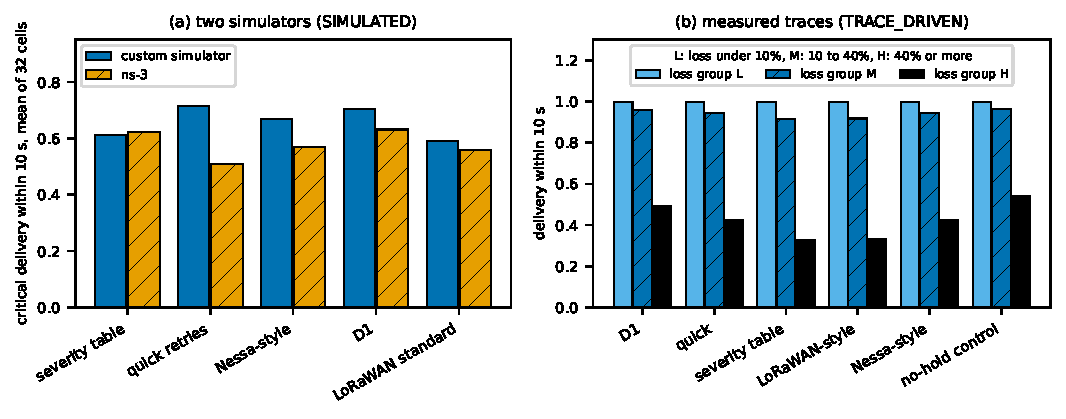
\includegraphics[width=\textwidth]{figures/vf_sim.pdf}
\caption{C6: (a) mean critical delivery within 10 s over \CellsN{} cells in the custom simulator and in ns-3 (SIMULATED); (b) delivery within 10 s on measured links by loss group (TRACE\_DRIVEN, \TOneN{} held-out devices).}\label{fig:sim}\end{figure*}
\emph{Trace caveats.} Frame-counter gaps measure gateway reception, not link loss alone, at the devices' own uplink period. A replay maps attempt $j$ of an alert to the reception state of the $j$-th next frame of the same device, whatever the real spacing between those frames; this assumes that consecutive frames stand for consecutive attempts and says nothing about loss at a shorter time scale. The sequences are gateway-reception sequences of weak links, not a crash-alert deployment. The held-out population is dominated by weak links: \TOneShareH\% of the devices have loss of 40\% or more, the median device loses \LinkMedLoss\% of its frames, the lag-1 autocorrelation of loss is \LinkAuto{}, and a frame after a lost frame is lost with probability \LinkCond{} against a pooled rate of \LinkPooled{}. Downlink loss is not measured; it is modelled as symmetric with the link loss rate. The duty limit in every simulation is 1\% unless a cell states another, which is stricter than the 10\% duty cycle that the Indian rules allow in the 433.05 to 434.79 MHz band~\cite{gsr347}; the LoED traces come from a different band and region.

\subsection{C7: deployment requirements}
\label{sec:c7}
\textbf{Simulated hardware-format logs.} The code was run on simulated hardware-format logs generated from stated sensor and link models (SIMULATED\_HW\_FORMAT). These are sanity checks of the code against the generator's assumptions, not findings about vehicles: the accuracies, the false-alarm rate and the latency below follow from those assumptions. The impact-side rule drops below 0.90 accuracy in \ShSideBelow{} of 16 variants: the side accuracy is \ShFlipAcc{} when the sign of the x axis is flipped and \ShHzAcc{} at 10 Hz sampling (Fig.~\ref{fig:deploy}). The 2 g trigger alone has a false-alarm rate of \ShFar{} on bench non-crash events. Confirmation by the vibration switches removes a fraction \ShSwRed{} of the false alarms and costs \ShSwLoss{} of the crash recall; the preregistered criterion was not met. The modelled trigger-to-acknowledgement latency is about \ShLatency{} ms for a 250 ms window, a 97-byte alert and a 26-byte acknowledgement at SF7, so a sub-500 ms claim fails for this configuration.

\textbf{Mounting calibration (L1, V16).} Rotating the samples into the vehicle frame from a still period and a straight braking or acceleration (GPS speed) restores the impact-side rule under tilts, yaws and 180-degree rotations: side accuracy \RFiveOneAcc{} against \RFiveOneRaw{} on the raw axes in simulated logs, and balanced front-against-side accuracy \RFiveOneNhtsa{} against \RFiveOneNhtsaRaw{} on real NHTSA pulses under synthetic rotations (the rotations and the calibration drive are synthetic). The method is standard \cite{Liu2022_isprs,Jameian2021_rsn}; only its measured effect on the side rule is claimed. It does not recover mirror-image axis flips (accuracy \RFiveMirrorAcc{}), which are not rotations. A test that detects mirror flips from turns (L11, added after the initial session of V16 and tested in its own family) detects them when both the accelerometer and the gyroscope are flipped (\RFiveElevenMir\% of \RFiveElevenN{} installations, \RFiveElevenFd\% false detections; descriptive) but only \RFiveElevenAccX\% (x) and \RFiveElevenAccY\% (y) for accelerometer-only flips against 95\% required, so it is not supported and the limit of L1 stays.
\begin{figure}[t]\centering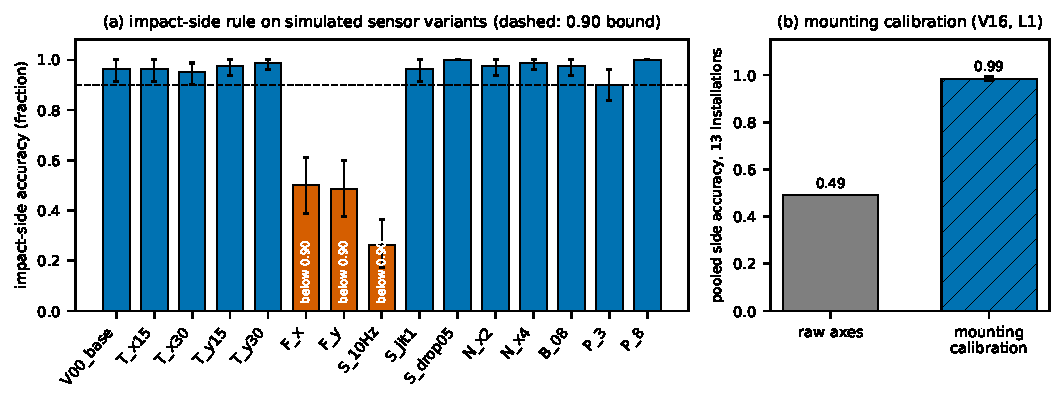
\includegraphics[width=\columnwidth]{figures/vf_deploy.pdf}
\caption{C7: (a) impact-side accuracy of the repository rule on 15 simulated sensor variants (SIMULATED\_HW\_FORMAT); (b) pooled side accuracy on raw axes and after the mounting calibration (SIMULATED\_HW\_FORMAT, 95\% interval over installations).}\label{fig:deploy}\end{figure}

\textbf{Wake-on-motion (L3, V16).} An accelerometer-only mode, in which the sensor's sample buffer collects data while the gyroscope is off in idle, keeps detection (recall \RFiveThreeRecB{} against \RFiveThreeRecA{} always on, at the 1\% target; a higher recall is not claimed) and, with datasheet currents and an active share of \RFiveThreeShare{} measured on VZCrash clips, lowers the estimated sensor and processor current to \RFiveThreeRatio{} of the always-on value (MEASURED\_SOFTWARE for detection, ANALYTICAL for energy). The active share comes from dataset clips and is probably higher than in a parked or cruising vehicle, so the ratio is a bound for busy driving and not a battery-life figure.

\subsection{C8: constrained-node alerting (round 6)}
\label{sec:c8}
\textbf{Micro-confirm (R6-1, SIMULATED and TRACE\_DRIVEN).} After the base has acknowledged the provisional frame, the node sends an 8-byte micro-confirm or micro-cancel (a one-byte pending index and a 7-byte core) whose 5-byte tag is HMAC-SHA256 over a letter, the provisional frame's tag, two content bytes and the boot counter; without an acknowledged provisional frame, or after the pending entry has expired, it sends the full frames as before. The ns-3 LoRaWAN module needs at least \RSixNsFrameBytes{} bytes, so the simulated frame has \RSixNsFrameBytes{} bytes against the 8-byte design, which stays within the evaluated size so that the airtime results are conservative for it; at SF7 it has the airtime of the 14-byte flash, so the simulated saving is against the 97-byte confirm only and the design frame would be shorter. Against the stored runs of the same seeds, the micro scheme uses \RSixAirOverRThreeLo{} to \RSixAirOverRThreeHi{} of the airtime of the two-stage alert in all sixteen ns-3 cells, and at most \RSixNinePerDelivHi{} of its airtime per delivered alert at SF9; delivery differs from the two-stage alert's by at most \RSixDeliveryGapMax{} and the lowest lower 95\% limit of the difference is \RSixDeliveryLowerMin{}. Delivery is supported in the sixteen ns-3 cells only: on the LoED traces the difference is zero by construction, because loss depends on the frame index and not on the frame length, so the trace groups are not evidence for delivery (their airtime ratios are \RSixTraceAirLowL{} for the low-loss group and \RSixTraceAirHighH{} for the high-loss group). The 40\% criterion on the extra airtime against the single-stage alert was nearly automatic, because the micro-confirm replaces the 97-byte confirm; that extra airtime is not offered as a gain, and the airtime over the two-stage alert is the informative number. The price is content: the micro-confirm carries no delta-V, peak or telemetry. The index, which the base assigns in the acknowledgement of the provisional frame, names the pending entry, so the base verifies the tag under one entry and the forgery probability stays at the single-entry value of $2^{-40}$ per frame: the expected time to one forgery is \FrameForgeOne{} years at the attacker's ceiling of 36 s of airtime per hour at SF7 (a lookup by trial would cut it to \FrameForgeSixty{} years for 60 pending entries and was rejected; ANALYTICAL; supplement).

\textbf{Formal results (R6-1c, R6-3a, FORMAL).} In ProVerif and Tamarin (symbolic, per-vehicle key, key reveal) the micro-confirm is accepted only when it binds to a provisional frame of the same vehicle, cannot be replayed onto another frame or vehicle, and a micro-cancel cannot be forged from another vehicle's key; a control model whose tag omits the provisional frame's tag is attacked in both tools. The proofs assume that the base selects the pending entry by vehicle and provisional tag, which the 8-byte frame replaces by a pending index; index variants of both models, with an index chosen by the attacker, are proved as well (supplement, abstraction table). In ProVerif, a hash ratchet keeps the authenticity and secrecy of past alerts after a later key is revealed, within a bound of \RSixRatchetSteps{} ratchet steps; the bound is part of the result, the Tamarin ratchet model of V16 ran out of memory, and no frame of the layout carries a ratchet step. The quarantine result (R6-3b) is in Section~\ref{sec:c4}. The symbolic models say nothing about implementation faults or side channels.

\textbf{Sequential early exit (R6-2, MEASURED\_SOFTWARE).} A running log-likelihood-ratio rule over the per-length forest scores, with thresholds chosen on validation data at the fixed rule's false-alarm rate, decides \RSixSeqGain{} ms earlier on average than the fixed rule (the early-exit rule of the two-stage alert with fixed thresholds) on \RSixHeldEvents{} held-out events (lower 95\% limit \RSixSeqGainLo{} ms) and raises the share of withdrawn provisional alerts by \RSixSeqRetractRise{} points (upper limit \RSixSeqRetractHi{} points). The preregistration quoted the fixed rule's mean decision time as \RSixPreregLo{} to \RSixPreregHi{} ms; on validation and held-out data it is \RSixFixedMeanMs{} ms (median \RSixFixedMedMs{} ms), so a gain of 200 ms was out of reach by arithmetic. The hypotheses were kept as written and the error is disclosed; neither hypothesis is supported.

\textbf{Footprint (R6-4, MEASURED\_SOFTWARE build artifacts).} The decision path was built for the target of the profile: the 15-tree forest of the headline detector (not the 16-bit compact variant of C3, whose flash is an estimate) is \RSixForestBytes{} bytes of constant data in flash, the HMAC code path is \RSixHmacCodeBytes{} bytes of code, the linked image is \RSixFlashBytes{} bytes of flash and the stack of the micro-confirm check sums to \RSixStackChain{} bytes over its call chain. The linked figure includes unused functions, because the linker of the toolchain stopped under garbage collection of sections, so the per-function sizes give the used path. Executed instructions, timing and energy are NOT\_RUN: no emulator for the target was available. These are build artifacts, not board measurements.

\textbf{Bounds and a retry proposition (R6-5, R6-7, ANALYTICAL).} The extra airtime of the two-stage alert has a lower bound of \RSixBoundSevenR{} at SF7 and \RSixBoundNineR{} at SF9 before any retry or collision; the micro scheme's airtime per provisional alarm is \RSixMicroOverRNine{} of the two-stage alert's at SF9. Under independent attempts with a non-decreasing earliest start, sending each attempt at its earliest feasible time is dominant under the stated assumptions; the traces are the check and agree with it. One gating rule follows: send two-stage alerts up to the spreading factor at which two gates hold, and the single-stage alert above it. The load gate is the lower bound times the measured retry and collision inflation within the 40\% budget (SF7 passes and SF9 fails in the two cells run). The lockout gate matters only in a region that enforces a per-transmission off-time on one sub-band, where the flash airtime must not exceed $d\,(T_F - s_f)$ (Section~\ref{sec:c5}); under the evaluated hourly allowance it is open at every spreading factor, so the rule gives SF7, and in a 1\% off-time region it gives none. This is a design rule, an interpolation from two simulated cells and the analysis, not a tested hypothesis.

\textbf{Scope.} This is an observability and sufficiency evaluation for single-point low-cost sensing: none of the estimators tested recovers pole and side impacts, and the results say what the sensor and the link allow, not what a vehicle deployment achieves. Of the seven hypotheses of round 6, \RSixSupp{} are supported.

\section{Negative results}
\label{sec:neg}
Table~\ref{tab:neg} lists the main hypotheses that did not hold. Each is a regime boundary: it says where an idea stops paying off under the stated profile, not that the idea is wrong everywhere. All \LedgerNot{} not-supported hypotheses and \LedgerPartly{} partly supported ones, grouped by layer with their likely mechanism, are in the release archive (negatives by layer, \texttt{supplementary\_full/}), and the ledger in the supplement gives the verdict of each. Original verdicts are not softened; a mechanism marked (inferred) was not tested.
\begin{table*}[t]\centering\caption{Main negative results: version, hypothesis, expectation, finding and likely mechanism.}\label{tab:neg}\small
\begin{tabular}{p{1.0cm}p{3.1cm}p{3.1cm}p{4.9cm}p{4.2cm}}\toprule
Version & Hypothesis & Expected & Found (label) & Likely mechanism\\\midrule
V4, V5, V7 & Direct severity classifier, anchored interval, abstention, augmentation (and their repeats) & gains over the anchored estimator & no gain in any repeat (MEASURED\_SOFTWARE) & small sealed fold; weak reliability score (inferred)\\
V5 & Physical and family pulse generators & pass a realism gate (area under the ROC curve $\le$ 0.60) & smallest point AUC \NegGateAuc{}; none passed (SIMULATED) & discriminable fine structure (inferred); a surrogate discriminator reaches \NegSurrAuc{}\\
V2, V5 & Burst variants, slotted fast path, listen-before-talk, relay & gain 5 points in burst cells & no gain; the slotted path worse by more than 2 points in \NegSlotLose{} of 16 cells (SIMULATED) & waiting for a slot; hidden terminals (inferred)\\
V7 & Overhear-and-suppress retries (OS-DR) & gain 5 points in 60\% of cells & gain in \NegOsdrGain{} of 32 cells, loss of more than 2 points in \NegOsdrLose{} (SIMULATED) & overheard frames are rare at the assumed load (inferred)\\
V11 & Short frame (R2) & gain 5 points over 97 bytes & gain in \RTwoCells{} of 16 cells, $p=$ \RTwoP{} (SIMULATED) & variance across cells (inferred)\\
V12 & Adaptive retry table (D1) & better than the severity table in any simulator & \XCustomDOneGain{} custom, \XNsDOneGain{} ns-3; a no-hold control beats it on traces & retry timing, not a mechanism\\
V15 & Short repeated provisional frame (A1) & extra airtime at SF9 at most 40\% and provisional delivery up 3 points & extra airtime \AOneAirNine{} at SF9 against \AOneAirNineR{} for the 14-byte frame, provisional delivery up \AOneProv{} points on fresh sniffer links (SIMULATED, TRACE\_DRIVEN) & a 24-byte frame costs more airtime; repeats add channel load (inferred)\\
V15 & Receiver diversity (A2) & two receivers add 10 points on weak links & up \ATwoGain{} points; \ATwoOne\% of devices are heard by one gateway only (exploratory) & a second gateway cannot help a device it does not hear\\
V16 & Post-event corroboration (L2) & near-miss false alarms down 25\% at equal recall & rate \RFiveTwoFa{} against \RFiveTwoFaBase{} (MEASURED\_SOFTWARE) & the confirm stage already holds the rate (inferred)\\
V16 & Threshold co-design with the network delay (L5) & 10\% lower 90th percentile of the time to awareness & no change in any of three link models & confirm stage fixed; small grid (inferred)\\
V16 & Crash-weighted gateway placement (L6) & 10 points more held-out crashes covered & \RFiveSixKTwo{} points at k = 200 and \RFiveSixKFour{} at k = 400 & placements overlap in cities (inferred)\\
V16 & Ratchet proofs (L7a) and flood containment (L8b) & forward secrecy proved; no legitimate vehicle quarantined & Tamarin heap exhausted; \RFiveEightQuar{} of 2,000 vehicle-hours quarantined & model size; per-minute spacing rule\\
V17 & Sequential early exit (R6-2) & 200 ms earlier with at most 2 points more retractions & \RSixSeqGain{} ms earlier; retractions up \RSixSeqRetractRise{} points (MEASURED\_SOFTWARE) & the fixed rule already decides early (mean \RSixFixedMeanMs{} ms), so little is left to gain\\
V18 & Reserved airtime budget under ACK suppression (H-R7-A1) & follow-up within D\_max in at least 99\% of runs at the load that exhausts the shipped policy & \RsevAoneRateOneResSfSeven\%, \RsevAoneRateOneResSfEight\% and \RsevAoneRateOneResSfNine\% at SF7, SF8, SF9 under a 1\% allowance (SIMULATED); every run at 10\% and under the off-time & earlier follow-ups spend the reserve; a reserve for four events restores 100\% (post-run, not in the family)\\
V18 & Benign cost of the reserve (H-R7-A2) & delivery down at most 1 point on the measured traces & down \RsevATwoHTenDelta{} points in the high-loss group under a 10\% off-time (TRACE\_DRIVEN); median time unchanged & the time reserve admits \RsevTtenFlashTriesSfSeven{} flash tries instead of four at SF7\\
V19 & Reserve for four events under ACK suppression (H-R7b-1) & follow-up on time in at least 99\% of runs, every cell, fresh seeds & lower limit \RsevbWorstLower\% in \RsevbCellsFeasible{} cells (SIMULATED); supported & chosen from round-7 data, so a confirmation and not a blind test\\
V19 & Benign cost of the four-event reserve (H-R7b-2) & delivery down at most 1 point and median time up at most 10\% on the traces, fresh start points & down \RsevbBenignHTenDelta{} points in the high-loss group under a 10\% off-time (TRACE\_DRIVEN); not supported & the time reserve does not depend on the size of the reserve\\
V18 & Pseudonym collisions (H-R7-B2) & collision probability at most $10^{-6}$ per frame at 1,000 vehicles and a window of 16 & \RsevBtwoLTwo{} at 2 bytes and \RsevBtwoLFour{} at 4 bytes (ANALYTICAL) & the bound needs \RsevBtwoLMeet{} bytes; the tag decides a collision\\
V16 & Mirror-flip detection (L11, own family) & 95\% for five flip types & \RFiveElevenAccX\% and \RFiveElevenAccY\% for accelerometer-only x and y flips & one of two estimates changes; short clips (inferred)\\
V2, V3 & Trigger cascade, group-aware training, conformal guarantee, class rule on delta-V, prevalence-adaptive threshold & recall or precision gains & no gain beyond the interval, or a rise in under-estimation (MEASURED\_SOFTWARE) & the 2 g trigger already passes most crashes; non-exchangeable splits (inferred)\\\bottomrule\end{tabular}\end{table*}

\section{Threats to validity}
\label{sec:threats}
\textbf{No physical hardware.} Every result is a statement about code run on data, simulations, traces, proofs or formulas. The firmware decision path was compared only in a host build. \textbf{Simulator dependence.} The D1 verdict changes between simulators and the calibration did not meet its criterion; the two-stage alert was run in ns-3 with a local patch. \textbf{Class pairs and models.} The pool of crash class pairs is finite; the reduced model bounds cover three vehicles; the Nessa-style baseline is an interpretation of a secondary description, because the full text of that paper was not available. \textbf{Searches.} Google Scholar and Scopus were not searched, and several cited works were read at abstract or record level (literature log in the release archive). \textbf{Data.} Crash-test pulses are severe and not representative of all crashes; VZCrash has no vehicle identifier; LoED frame-counter gaps measure gateway reception, and most held-out devices are weak links. \textbf{Transmit power.} The stored link results assume 14 dBm; a compliant dipole node transmits at most \RsevbPowerMaxDipole{} dBm, so they are optimistic on margin by up to \RsevbPowerExtraDb{} dB. \textbf{Base behaviour.} Acknowledgement only after the tag verifies, and an atomic seen-set check and insert, are properties of the reference base code and design requirements for a base server; no base server exists, the ns-3 gateway acknowledges every received frame, and a keyless replay of a valid frame is re-acknowledged and consumes downlink budget unless the base meets R-REACK. \textbf{Regulation.} The Indian rules for 433.05 to 434.79 MHz leave the observation interval of the 10\% duty cycle undefined and give no channel plan; the evaluation was run under a stricter 1\% hourly allowance, and a deployed node would need type approval under rule 5~\cite{gsr347}. \textbf{Formal models.} Jamming, key provisioning and revocation, compromise of the base master key and the replay after a base reboot are outside the models (the last is found as a trace). Tamarin, ProVerif and the enumeration are symbolic and single-link; one reboot lemma was not decided for the frozen design; the freshness field of the 14-byte provisional frame is not modelled, the proofs hold at the level of the message structure stated in the abstraction table, and the byte layout of the supplement is a design proposal that no firmware implements. \textbf{Duty model.} A per-transmission off-time was not evaluated; the stored two-stage results do not transfer to a region that enforces one on a single sub-band. \textbf{Retry queue.} The evaluated node can leave the base in the provisional state when every frame of the final stage is lost, because the code has no base timeout.

\section{Conclusion}
\label{sec:concl}
For a crash-alert node on a constrained LPWAN link the study gives requirements, not a validated product: duplicates must be removed from the benchmark, the sensor range must match the crash mode, the acknowledgement must be bound to the vehicle, a car should keep a boot counter, a provisional frame must not carry a severity class and costs more airtime at SF9 unless the confirm is replaced by a micro-confirm that is bound to it, and, on isolated weak links in single-link replays, the number of attempts that fit before the deadline governed delivery, with retry spacing not represented in the replay (the ns-3 runs do not show the same ranking). No measurement on physical hardware is reported; results are from public crash and naturalistic datasets, public LoRaWAN traces, two network simulators, formal models and simulated hardware-format logs. The estimators tested do not recover pole and side impacts, and the formal results are symbolic. Future work is a bench run of the two-stage alert and of the micro-confirm with the frame layout of the supplement, a run under a per-transmission off-time, ns-3 support for SF11, hardware logs, and a Scopus search.

\section*{Data and code availability}
Code: Apache-2.0, in the repository with a pinned environment, the formal models, the ns-3 patch, the preregistrations, the hypothesis ledger and the result files. Derived data from VZCrash are released under CC BY-NC 4.0 with attribution; raw third-party data are not redistributed. NHTSA crash-test data and FARS files are public; LoED, the LoRaWAN sniffer set, GeoNames and UCI HAR are CC BY 4.0; SisFall is available from its authors \cite{Sucerquia2017_sisfall}; it is not redistributed with this artefact because no data licence is stated (a Zenodo copy states CC BY 4.0 but names no creators, so we did not rely on it; see \texttt{scripts/fetch\_sisfall.md}). File hashes, access dates and licences are in the supplement. A Zenodo DOI for the code and derived data: [to be filled by the author].

\section*{Acknowledgement, contributions, funding, interests and AI tools}
Acknowledgement: the VZCrash authors confirmed the duplicate finding; [wording to be confirmed by the author]. Author contributions (CRediT): [to be filled by the author]. Funding: [to be filled by the author]. Competing interests: [to be filled by the author]. Use of AI tools: an AI coding assistant (Anthropic Claude, through the Claude Code tool) was used to write and run analysis code and to draft parts of the text and of the supplement under the author's direction; the author checked the results. IEEE Access asks that AI-generated text is disclosed here and that each section with such text cites the system used: [the author must list the sections and confirm the citation form].

\bibliographystyle{IEEEtran}
\bibliography{references}

\EOD
\end{document}
